
\ifdefined\ishandout
\documentclass[11pt,english,handout]{beamer}
\else
\documentclass[11pt,english]{beamer}
\fi

%\documentclass[11pt]{beamer}
\usepackage{mathptmx}
\renewcommand{\sfdefault}{lmss}
\renewcommand{\familydefault}{\sfdefault}
\usepackage[T1]{fontenc}
\usepackage[latin9]{inputenc}
\usepackage{amsmath}
\usepackage{amssymb}
\usepackage{graphicx}
\usepackage{xcolor,multirow,colortbl}
\PassOptionsToPackage{normalem}{ulem}
\usepackage{ulem}
\usepackage{caption}
\captionsetup{labelformat=empty}
\usepackage{bbm}
\usepackage{upgreek}
\usepackage{graphicx}
\setbeamertemplate{section in toc}[sections numbered]
\makeatletter
\usepackage{caption} 
\usepackage{bm}
\usepackage{subfig}
\captionsetup[table]{skip=10pt}
%%%%%%%%%%%%%%%%%%%%%%%%%%%%%% Textclass specific LaTeX commands.
% this default might be overridden by plain title style
\newcommand\makebeamertitle{\frame{\maketitle}}%
% (ERT) argument for the TOC
\AtBeginDocument{%
	\let\origtableofcontents=\tableofcontents
	\def\tableofcontents{\@ifnextchar[{\origtableofcontents}{\gobbletableofcontents}}
	\def\gobbletableofcontents#1{\origtableofcontents}
}

%%%%%%%%%%%%%%%%%%%%%%%%%%%%%% User specified LaTeX commands.
%\documentclass[presentation]{beamer}


\def\Tiny{\fontsize{7pt}{8pt}\selectfont}
\def\Normal{\fontsize{8pt}{10pt}\selectfont}

\usetheme{Madrid}
\usecolortheme{lily}
%\setbeamercovered{transparent}
\useinnertheme{rounded}


\setbeamertemplate{footline}{\hfill\Normal{\insertframenumber/\inserttotalframenumber}}
%\setbeamertemplate{footline}{}

\setbeamertemplate{navigation symbols}{}

\newenvironment{changemargin}[2]{%
	\begin{list}{}{%
			\setlength{\topsep}{0pt}%
			\setlength{\leftmargin}{#1}%
			\setlength{\rightmargin}{#2}%
			\setlength{\listparindent}{\parindent}%
			\setlength{\itemindent}{\parindent}%
			\setlength{\parsep}{\parskip}% 
		}%
		\item[]}{\end{list}}

\setbeamertemplate{footline}{\hfill\insertframenumber/\inserttotalframenumber}
\setbeamertemplate{navigation symbols}{}

%\usepackage{times}  % fonts are up to you
\usepackage{graphicx}
%\usepackage{graphics}
\usepackage{epsfig}
\usepackage{bm}
\usepackage{epsf}
\usepackage{float}
\usepackage[final]{pdfpages}
\usepackage{multirow}
\usepackage{colortbl}
\usepackage{xkeyval}
%\usepackage{sgame}
%\usepackage{pst-node}
\usepackage{listings}
\usepackage{ifthen}
%\usepackage{hyperref}
\usepackage{tikz}

%\usepackage{times}  % fonts are up to you
%\usepackage{graphicx}
%\usepackage{graphics}
\usepackage{epsfig,bm,epsf,float}
\usepackage[final]{pdfpages}
\usepackage{xcolor,multirow,colortbl}
\usepackage{xkeyval}
\usepackage{verbatim}
%\usepackage{sgame}
%\usepackage{pst-node}
\usepackage{listings}
%\usepackage{handoutWithNotes}
%\pgfpagesuselayout{3 on 1 with notes}[letterpaper,border shrink=5mm]
%\pgfpagesuselayout{2 on 1 with notes landscape}[letterpaper,border shrink=5mm]
\usepackage{setspace}
\usepackage{ragged2e}

\setbeamersize{text margin left=1em,text margin right=1em} % CambridgeUS spacing if you use default instead


%\pdfmapfile{+sansmathaccent.map}

% Table formatting
\usepackage{booktabs}


% Decimal align
\usepackage{dcolumn}
\newcolumntype{d}[0]{D{.}{.}{5}}


\global\long\def\expec#1{\mathbb{E}\left[#1\right]}
\global\long\def\var#1{\mathrm{Var}\left[#1\right]}
\global\long\def\cov#1{\mathrm{Cov}\left[#1\right]}
\global\long\def\prob#1{\mathrm{Prob}\left[#1\right]}
\global\long\def\one{\mathbf{1}}
\global\long\def\diag{\operatorname{diag}}
\global\long\def\expe#1#2{\mathbb{E}_{#1}\left[#2\right]}
\DeclareMathOperator*{\plim}{\text{plim}}

%\usefonttheme[onlymath]{serif}

\usepackage{appendixnumberbeamer}
\renewcommand{\thefootnote}{}

\setbeamertemplate{footline}
{
	\leavevmode%
	%   \hbox{%
	%      \begin{beamercolorbox}[wd=\paperwidth,ht=2.25ex,dp=1ex,right]{date in head/foot}%
	%\usebeamerfont{date in head/foot}\insertshortdate{}\hspace*{2em}%
	\hfill
	%turning the next line into a comment, erases the frame numbers
	\insertframenumber{}\hspace*{2ex}\vspace{1ex}
	
	%    \end{beamercolorbox}}%
}

\definecolor{blue}{RGB}{0, 0, 210}
\definecolor{red}{RGB}{170, 0, 0}

\makeatother

\usepackage[english]{babel}

\usepackage{tikz}
\newcommand*\circled[1]{\tikz[baseline=(char.base)]{             \node[circle,ball color=structure.fg, shade,   color=white,inner sep=1.2pt] (char) {\tiny #1};}} 

\makeatletter
\let\save@measuring@true\measuring@true
\def\measuring@true{%
	\save@measuring@true
	\def\beamer@sortzero##1{\beamer@ifnextcharospec{\beamer@sortzeroread{##1}}{}}%
	\def\beamer@sortzeroread##1<##2>{}%
	\def\beamer@finalnospec{}%
}
\makeatother

\definecolor{amethyst}{rgb}{0.6, 0.4, 0.8}

\setbeamersize{text margin left= .8em,text margin right=1em} 
\newenvironment{wideitemize}{\itemize\addtolength{\itemsep}{10pt}}{\enditemize}
\newenvironment{wideitemizeshort}{\itemize}{\enditemize}

\newcommand{\indep}{\perp\!\!\!\!\perp} 


\DeclareMathOperator*{\argmax}{arg\,max}
\DeclareMathOperator*{\argmin}{arg\,min}

\begin{document}
	
	%% Title slide
	\begin{frame}[noframenumbering]{}
		\vspace{0.5cm}
		\title[]{Chapter 5: Multivariate Regression}
		\author{Jonathan Roth}
		\date{Mathematical Econometrics I \\ Brown University\\} 
		\titlepage {\small{}\ }\thispagestyle{empty} \vspace{-30pt}
		
	\end{frame}
	
	
	\begin{frame}{Outline}

	1. Deriving Multivariate Regression and OLS
	\vspace{0.8cm}
	
	2. Regression and Causality
	\vspace{0.8cm}
	
	3. Regression Odds and Ends
	
	\end{frame}
		
	\begin{frame}{Moving Beyond One ``Regressor''}
		\begin{wideitemize}
			
			\item
			So far we've talked about regression as a way of approximating the CEF $E[Y_i|X_i =x ] \approx \alpha + x \beta $ for a single scalar $X_i$\smallskip
			\begin{itemize}
					\item 
					We then showed how the estimand ($\alpha$,$\beta$) can be estimated by OLS
				\end{itemize}
			
			\pause
			\item
			Next we'll see how this can be generalized to approximate/estimate $E[Y_i| \mathbf{X}_i =\mathbf{x} ] \approx \mathbf{x}' \bm{\beta}$ for a vector $ \mathbf{X_i} = (1,X_{i1},...,X_{iK})'$ 
				\begin{itemize}\smallskip
					\item 
					Note: As usual, I'll be putting vectors/matrices in bold type-face
				\end{itemize}
			
			\pause
			\item
			Two main motivations for this: \medskip
			\end{wideitemize}	

			\pause
\begin{enumerate}
			\item
			We want to use regression to identify causal effects, but conditional unconfoundedness is only plausible with multiple controls \smallskip
			\begin{itemize}
				\item 
				In the Brown/URI example, we may want to control for high school GPA, family income, SAT, race ...
			\end{itemize}
			\medskip
			
			\pause
			\item
			We want a \emph{nonlinear} CEF approx.: e.g. $E[Y_i\mid X_i]\approx\alpha+X_i\beta+X_i^2\gamma$ \smallskip
			\begin{itemize}
			\item We can ``trick`` regression into doing this by setting $\mathbf{X_i} = (1, X_{i}, X_{i}^2)'$
			\end{itemize}
			\end{enumerate}
			
		
		
	\end{frame}
	
		
	\begin{frame}{Log Wages by Age}
		\centering
		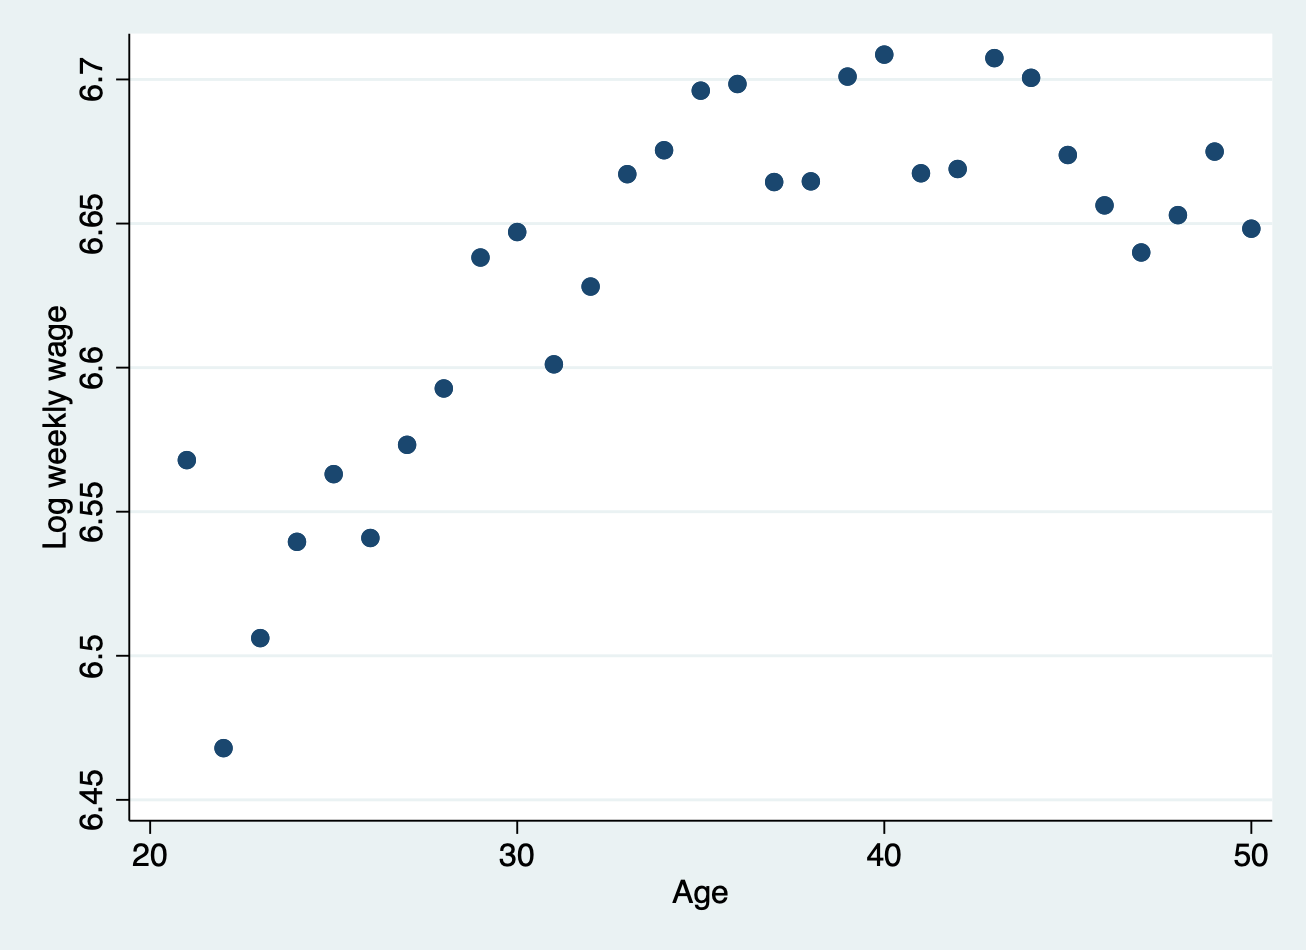
\includegraphics[width = 0.8 \linewidth]{logwages}
		
	\end{frame}
	
	\begin{frame}{OLS Regression (Linear Fit)}
		\centering
		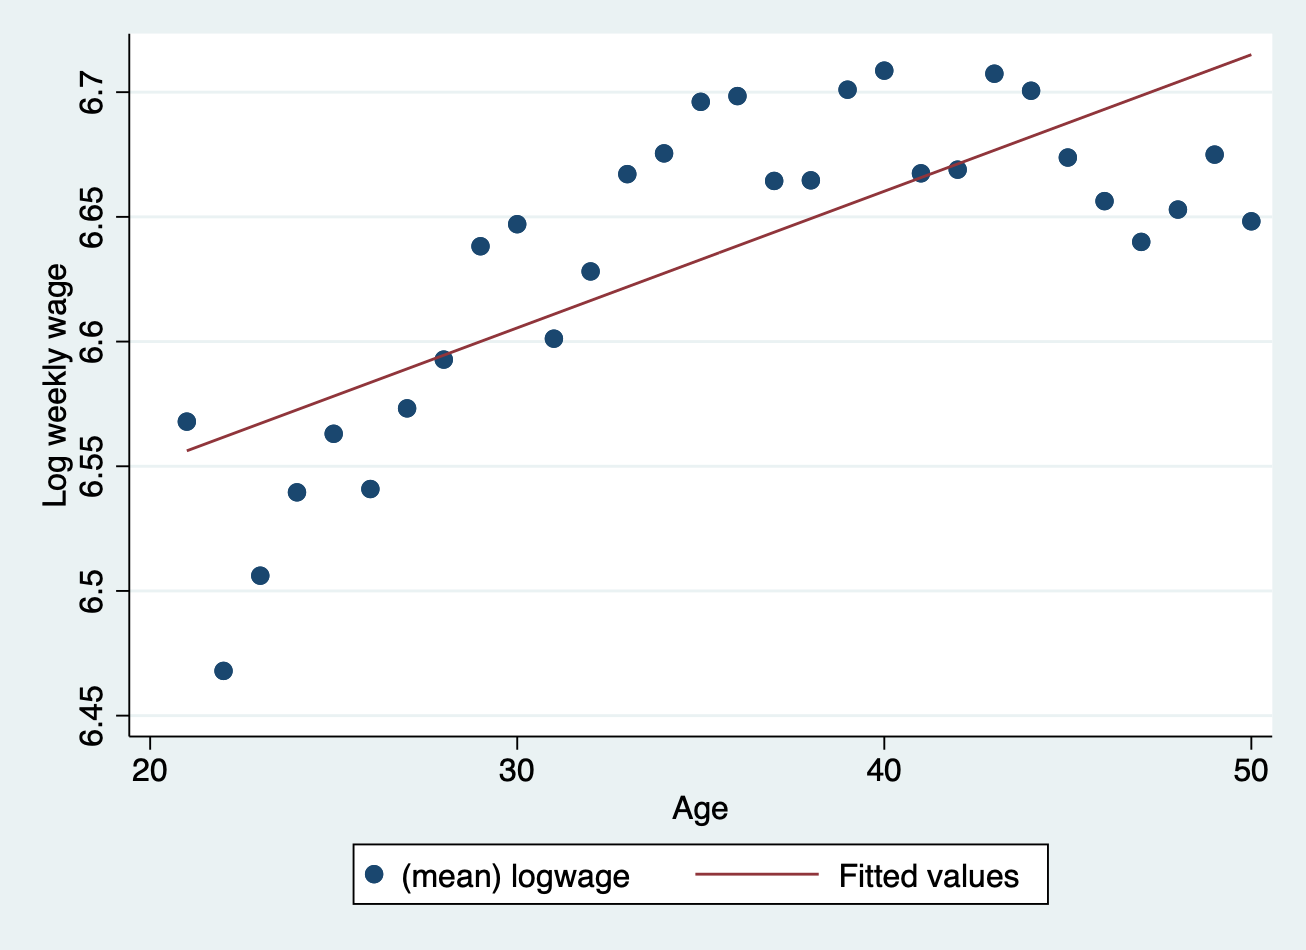
\includegraphics[width = 0.8 \linewidth]{logwages-linear}
		
	\end{frame}
	
		\begin{frame}{OLS Regression (Quadratic Fit)}
		\centering
		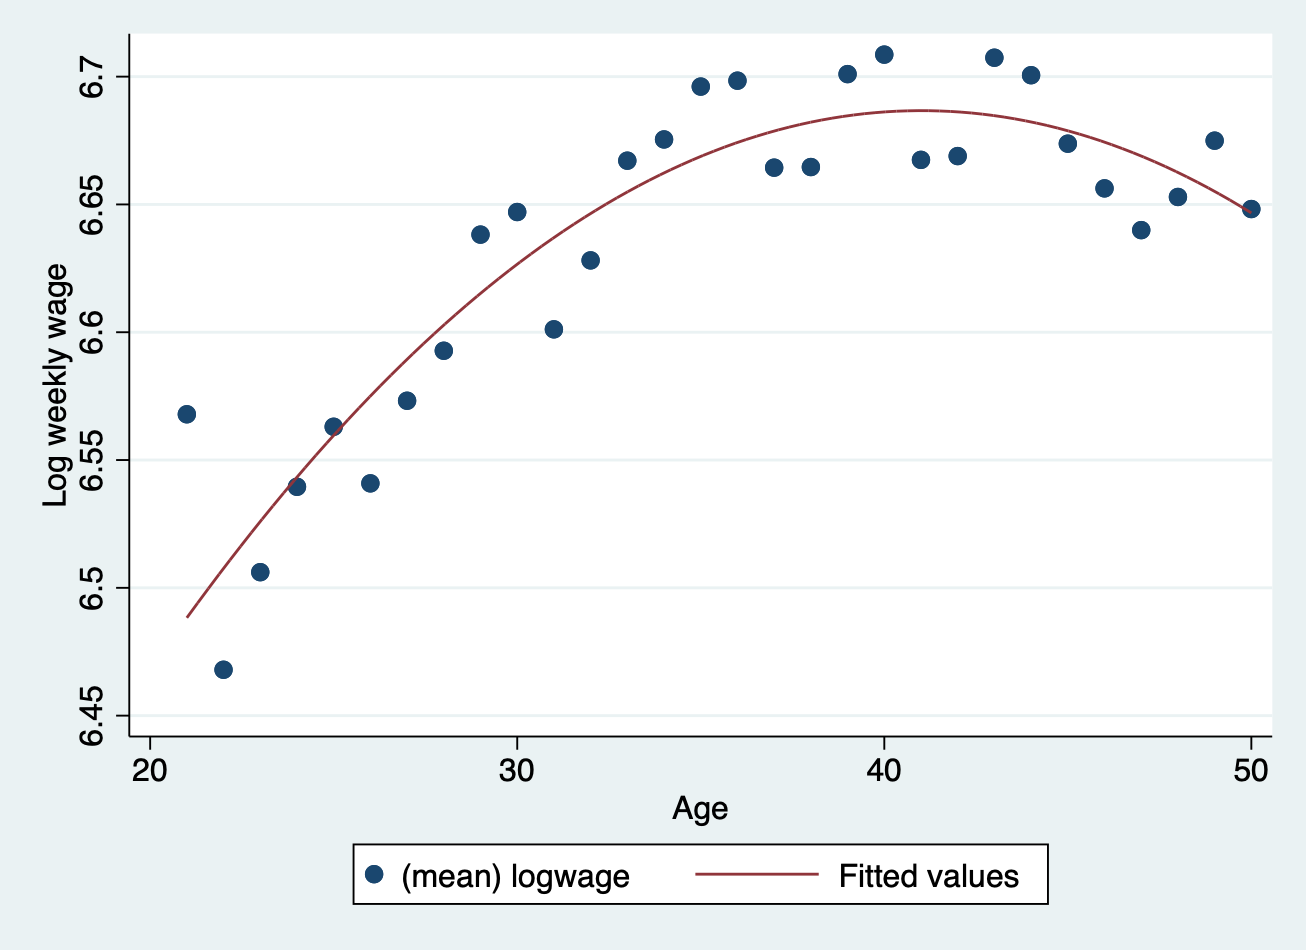
\includegraphics[width = 0.8 \linewidth]{logwages-quadratic}
		
	\end{frame}

\begin{frame}{Multivariate Regression as a Least-Squares Problem}
	\begin{wideitemize}
		\item
		Recall with univariate OLS we solved for 
		$$(\alpha, \beta) = \argmin_{a,b} E[ (Y_i - (a + b X_i))^2 ] $$
		
		We showed if the CEF is linear, then $E[Y|X] = \alpha + \beta X$; while if not, $\alpha + \beta X$ gave the best non-linear approximation
		
		\pause
		\item
		We will now consider the multi-variate analog:
		\begin{align*}
		\boldsymbol\beta= \arg \min_{\mathbf{b}} E\left[(Y_i-\mathbf{X}_i^\prime\boldsymbol b)^2\right]
		\end{align*}
	
		\item
		Using similar steps for the univariate case, we can show that if the CEF is linear in $\mathbf{X}$, then $E[Y| \mathbf{X}] = \mathbf{X}'\boldsymbol{\beta}$; if not, then $\mathbf{X}'\boldsymbol{\beta}$ is the MSE-minimizing approximation to the CEF.
	 
	\end{wideitemize}
\end{frame}
	
%	\begin{frame}{Multivariate Regression as a CEF Approximation}
%\vspace{0.1cm}
%		\begin{wideitemize}
%			\item
%			As before, let's consider the mean-squared error (MSE) minimizing linear approximation to the true CEF, $\mu(\mathbf{x})=E[Y_i\mid\mathbf{X}_i=\mathbf{x}]$:
%\begin{align*}
%\boldsymbol\beta= \arg \min_{\mathbf{b}} E\left[(\mu(\mathbf{X}_i)-\mathbf{X}_i^\prime\boldsymbol b)^2\right]
%\end{align*}
%
%\pause{}\vspace{-0.4cm}
%
%			\item How do we solve this without knowing $\mu(\mathbf{x})$? \pause{} As before, we can show 
%\begin{align*}
%\boldsymbol\beta= \arg \min_{\mathbf{b}} E\left[(Y_i-\mathbf{X}_i^\prime\boldsymbol b)^2\right]
%\end{align*}
%
%And then take FOC to solve for $\boldsymbol{\beta}$\pause{}\smallskip
%\item Proof for this equivalence again follows by LIE-ing:
%\begin{align*}
%E\left[(Y_i-\mathbf{X}_i^\prime\boldsymbol b)^2\right]=&E\left[((\mu(\mathbf{X}_i)-\mathbf{X}_i^\prime\boldsymbol b) + (Y_i- \mu(\mathbf{X}_i)))^2\right]\\
%\pause{}
%=&E\left[(\mu(\mathbf{X}_i)-\mathbf{X}_i^\prime\boldsymbol b)^2\right]+\underbrace{E\left[(Y_i- \mu(\mathbf{X}_i))^2\right]}_{\text{Doesn't depend on $\mathbf{b}$}}\\
%&+2 \underbrace{E\left[(\mu(\mathbf{X}_i)-\mathbf{X}_i^\prime\boldsymbol b)(Y_i- \mu(\mathbf{X}_i))\right]}_{\text{$=0$ by LIE}}
%\end{align*}
%so $\arg\min_{\textbf{b}} E\left[(Y_i-\mathbf{X}_i^\prime\boldsymbol b)^2\right]=\arg\min_{\textbf{b}} E\left[(\mu(\mathbf{X}_i)-\mathbf{X}_i^\prime\boldsymbol b)^2\right]$
%			 
%		\end{wideitemize}
%	\end{frame}
%	
	
	\begin{frame}{Solving for Regression Coefficients}
		\begin{wideitemize}
			\item
			So the \emph{population regression coefficient} $\boldsymbol\beta$ solves least squares problem
						
			$$\bm{\beta} = \argmin_{\mathbf{b}} E[ (Y_i - \mathbf{X}_i '\mathbf{b})^2]$$
			
			\pause
			\item
			To solve for $\bm{\beta}$, we take the derivative (i.e. gradient) and set it to zero
			\begin{align*}
				& \dfrac{d}{d \bm{\beta}} E[ (Y_i - \mathbf{X}_i '\bm{\beta})^2] = \mathbf{0} \pause{} \\
				\Rightarrow & E[ \dfrac{d}{d \bm{\beta}} (Y_i - \mathbf{X}_i '\bm{\beta})^2] = \mathbf{0} \pause{} \\
				\Rightarrow & E[-2 \mathbf{X}_i (Y_i - \mathbf{X}_i '\bm{\beta})] = \mathbf{0} \pause{}\\
				\Rightarrow & E[\mathbf{X}_i Y_i] = E[\mathbf{X}_i \mathbf{X}_i ']\bm{\beta}
			\end{align*}
		
	
		\end{wideitemize}
	\end{frame}
	
	
	\begin{frame}{Multivariate Regression, in the Population and Sample}
		\begin{wideitemize}
			\item
			Solving for $\bm{\beta}$, we obtain an expression involving population means:
			$$\bm{\beta} = E[ \bm{X}_i \bm{X}_i'  ]^{-1} E[\bm{X}_i Y_i] $$
			\vspace{-0.3cm}
			\begin{itemize}
			\item With a bit of algebra, you can show that this reduces to the bivariate formulas $\beta=\frac{Cov(X_i,Y_i)}{Var(X_i)}$ and $\alpha=E[Y_i]-E[X_i]\beta$ when $\mathbf{X}_i=(1,X_i)^\prime$
			\end{itemize}
			\pause\smallskip
			\item
			To estimate $\bm{\beta}$, we can replace population means with sample means. 
			
			\pause
			$$ \bm{\hat\beta} = \left( \frac{1}{N} \sum_{i=1}^N \bm{X}_i \bm{X}_i' \right)^{-1}  \left( \frac{1}{N} \sum_{i=1}^N \bm{X}_i Y_i \right)$$
			
			\pause\smallskip
			\item 
			We thus now have a general way of estimating $E[Y_i\mid \mathbf{X}_i]\approx \mathbf{X}_i^\prime\boldsymbol{\beta}$ for any vector $\mathbf{X}_i=(1,X_{i1},\dots,X_{iK})^\prime$ 
		\end{wideitemize}
	\end{frame}
	
	%Outline
	
	% Motivation

	% Example 1 --- multivariate regression
		
	% Mechanics of Multivariate Least-Squares
	
	% Interpreting coefficients
	
	% Example 2 -- multivariate controls. Dale and Krueger
		
	% Omitted variable bias
	
	% F-tests? 
	
		
	
	\begin{frame}{Quadratic Regression of Log Wages on Age} 
	\begin{center}
	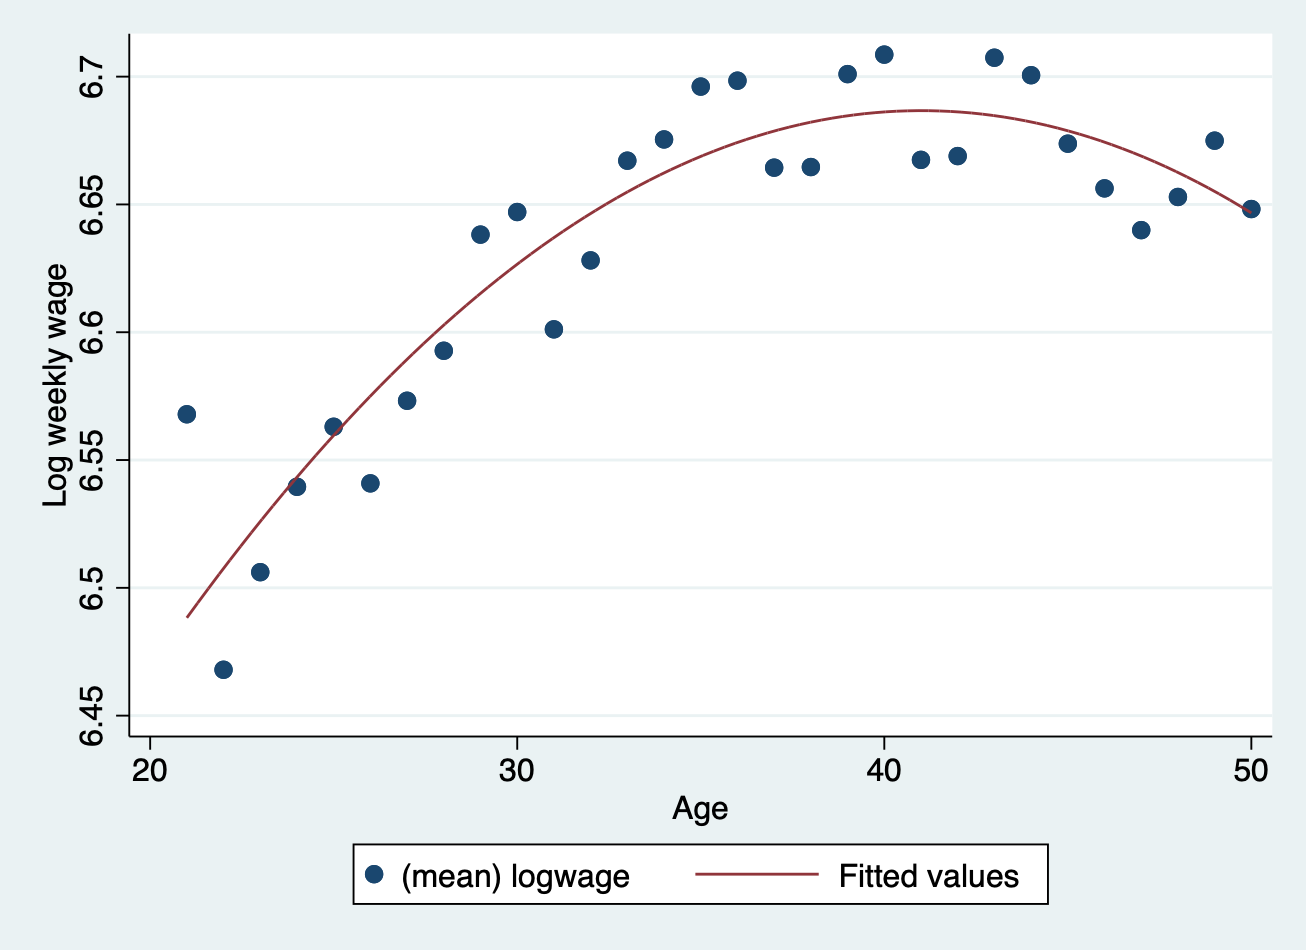
\includegraphics[width = 0.8 \linewidth]{logwages-quadratic}
	
	\begin{tabular}{lr}
	Constant & 5.8591 \\
	Age & 0.0403 \\
	Age$^2$ & -0.0005
	\end{tabular}
	
	\end{center}
	
	\end{frame}
	
	
	\begin{frame}{Interpreting Quadratic Regression Coefficients}
		\begin{itemize}
			\item 
			With a quadratic fit, we have 
			
			$$E[Y_i | X_i =x] \approx \bm{\hat\beta}_0 +  \bm{\hat\beta}_1 x + \bm{\hat\beta}_2 x^2$$
			\smallskip

			\pause
			\item
			What is the slope of $ E[Y_i | X_i  =x] $? Differentiating, we have \pause{}
			
			$$\dfrac{d}{dx} E[Y_i | X_i =x] \approx  \bm{\hat\beta}_1  + 2 \bm{\hat\beta}_2 x$$
			\smallskip

			
			\pause
			\item
			The estimated derivative from a multivariate regression, in this case $ \bm{\hat\beta}_1  + 2 \bm{\hat\beta}_2 x$, is sometimes called the ``marginal effect'' at $x$
				\smallskip

				\begin{itemize}
					\item 
					This terminology is a bit unfortunate: this need not be a \textit{causal} effect, just an estimated derivative of the CEF
				\end{itemize}
				
		\end{itemize}
	\end{frame}

\begin{frame}{Interpreting Our Example Coefficients}
		\begin{tabular}{lr}
		Constant ($\bm\hat\beta_0$) & 5.8591 \\
		Age ($\bm\hat\beta_1$) & 0.0403 \\
		Age$^2$ ($\bm\hat\beta_2$) & -0.0005
	\end{tabular}
\medskip
	
\begin{wideitemize}
	\item
	What is the estimated slope of average log-earnings w.r.t. age? \pause
	
	\item
	$\bm{\hat\beta_1} + 2 \bm{\hat\beta_2} \cdot Age \pause{} = 0.0403 - 2 \times 0.0005\cdot Age =  \pause{} 0.0403 - 0.001 \cdot Age$.
	
	\pause
	\item
	For what age is estimated earnings highest? \pause
	$$0.0403 - 0.001 \cdot Age = 0 \pause{} \Rightarrow Age = 0.0403 / 0.001 = 40.3 $$
	
\end{wideitemize}	
\end{frame}
	
	\begin{frame}{Re-Writing Multivariate OLS with Matrix Algebra}
		\begin{wideitemize}
		
		\item
		We showed that 
		$$ \bm{\hat\beta} = \left( \frac{1}{N} \sum_{i=1}^N \bm{X}_i \bm{X}_i' \right)^{-1}  \left( \frac{1}{N} \sum_{i=1}^N \bm{X}_i Y_i \right)$$
		
		\item
		This formula is often given more compactly with matrix notation.
		
		\pause
		\item
		Let $\bm{X}$ be an $N \times K$ matrix w/ $X_{ik}$ giving the element in row $i$ and column $k$. \pause Likewise let $\bm{Y} = (Y_1,...,Y_N)'$.
		
		\pause
		\item
		For example, if $\bm{X}_i = (1, X_i)'$ and $N=3$, then
		
		$$\bm{X} = \left( \begin{array}{rr} 1 & X_{1} \\ 1 & X_{2} \\ 1 & X_{3}   \end{array}  \right) \pause \hspace{2cm} \bm{Y} = \left( \begin{array}{r} Y_{1} \\Y_{2} \\ Y_{3}   \end{array}  \right)$$
		
		\pause
		\item
		Using this notation, one can show that $\bm{\hat\beta} = \left(\bm{X'X}\right)^{-1} \bm{X}'\bm{Y}$
	\end{wideitemize}	
		
	\end{frame}
	
	\begin{frame}{Asymptotic Properties of Multivariate OLS} 
		\begin{wideitemize}
			
		\item
		To test hypotheses about the population CEF, we need to derive the asymptotic distribution of $\bm{\hat\beta}$. 
		
		\pause
			
		\item
		As with univariate OLS, we can show that $\bm{\hat\beta}$ is consistent and asymptotically normally distributed.
		\pause
	
		\item
		The proofs are very similar to those for univariate OLS, so I'll skip them and show you the results!
		
		\pause
		\item
		\textbf{Consistency:} $\bm{\hat\beta} \rightarrow_p \bm{\beta}$.
		
		\end{wideitemize}
	\end{frame}

	\begin{frame}{Asymptotic Properties of Multivariate OLS} 
		\begin{wideitemize}
			\item
			\textbf{Asymptotic normality}:
			$$\sqrt{N} (\bm{\hat\beta} - \bm{\beta}) \rightarrow_d \mathrm{N}(0, \bm{\Sigma}),$$
			
			\noindent where $\bm{\Sigma} = E[ \bm{X}_i \bm{X}_i' ]^{-1} Var( \bm{X}_i \epsilon_i  )	E[ \bm{X}_i \bm{X}_i' ]^{-1} $ and $\epsilon_i = Y_i - \bm{X}_i' \bm{\beta}$
			
			
			\pause
			\item 
			We can estimate $\bm{\Sigma}$ by replacing population means with sample means	
			
			$$\bm{\hat\Sigma} = \left( \frac{1}{N} \sum_{i=1}^N \bm{X}_i \bm{X}_i' \right)^{-1} \left(\frac{1}{N} \sum_{i=1}^N \bm{X}_i \bm{X}_i' \hat\epsilon_i^2  \right) \left( \frac{1}{N} \sum_{i=1}^N \bm{X}_i \bm{X}_i' \right)^{-1}  $$
			
			where  $\hat\epsilon_i = Y_i - \bm{X}_i' \bm{\hat\beta}$.
			
			
			\item\pause{}
			Note: $\bm{\hat\Sigma}$ is a \textit{matrix}. 
				\begin{itemize}
					\item 
					The standard error for $\bm{\hat\beta}_j$ is $\sqrt{\bm{\hat\Sigma}_{jj}} / \sqrt{N}$
					
					\item
					The off-diagonal elements correspond with covariances between $\bm{\hat\beta}_j$,$\bm{\hat\beta}_k$
				\end{itemize}
			
		\end{wideitemize}
	\end{frame}

	\begin{frame}{Example - Log Earnings by Age} 
		
		\begin{tabular}{lrr}
			Variable & Coefficient & SE \\ \hline
			Constant ($\beta_0$) & 5.8591 & 0.1409 \\
			Age ($\beta_1$) & 0.0403 &  0.0077\\
			Age$^2$ ($\beta_2$) & -0.0005 & 0.0001
		\end{tabular}
\medskip
		
		
		\begin{wideitemize}
			\item
			What is a confidence interval for $\beta_2$? 
			
			\pause{}
			$$\hat\beta_2 \pm 1.96 \times SE_{\beta_2} = \pause{} -0.0005 \pm 1.96 \times 0.0001 \pause{} = [-0.0007, -0.0003]  $$
		\end{wideitemize}
	\end{frame}

% PH to here 10/16

	\begin{frame}{Controlling for Multiple Variables} 
		\begin{wideitemize}
			\item
			In addition to allowing for more flexible functional forms (e.g. quadratic), multivariate OLS allows us to approximate the CEF conditional on multiple variables at once
			
			\pause
			\item
			Example: we have data from Texas on each county's presidential vote over the last three elections (2012,2016,2020)
			
			\pause
			\item
			Let $Y_i = $ Biden vote share in county $i$, $X_{i1}$ = Clinton vote share in county $i$, and $X_{i2} = $ Obama vote share in county $i$
			
			\pause
			\item
			We estimate the regression 
			
			$$Y_i = \beta_0 + \beta_1 X_{i1} + \beta_2 X_{i2} + \epsilon_i$$
			
			\pause
			\item 
			This says that 
			$$\scriptsize  E[  \text{Biden vote} | \text{Clinton vote} , \text{Obama vote} ] \approx \beta_0 + \beta_1 \times \text{Clinton vote} + \beta_2 \times \text{Obama vote}  $$
		\end{wideitemize}	
	\end{frame}
	
	
	\begin{frame}{OLS Estimates}
		\begin{tabular}{lrr}
			Variable & Coefficient & SE \\ \hline
			Constant & 0.05 & 0.01 \\
			Clinton & 1.39 & 0.13 \\
			Obama & -0.56 & 0.13
		\end{tabular}
	\medskip 
	
	\pause
	\begin{wideitemize}
		\item
		What is the predicted Biden vote share for a county where Obama got half the vote and Clinton got 60\%?
		\pause
		$$\hat\beta_0 + \hat\beta_1 0.6 + \hat\beta_2 0.5 = \pause{} 0.05 + 1.39 \times 0.6 - 0.56 \times 0.5  = \pause{} 0.604$$
		\pause
\vspace{-0.5cm}
		\item
		Notice that the coefficient on Obama vote share is \textit{negative}
		\item
		Wait, does this mean Biden did worse in places that Obama did well?!
	\end{wideitemize}
	\end{frame}


	\begin{frame}
		\begin{center}
		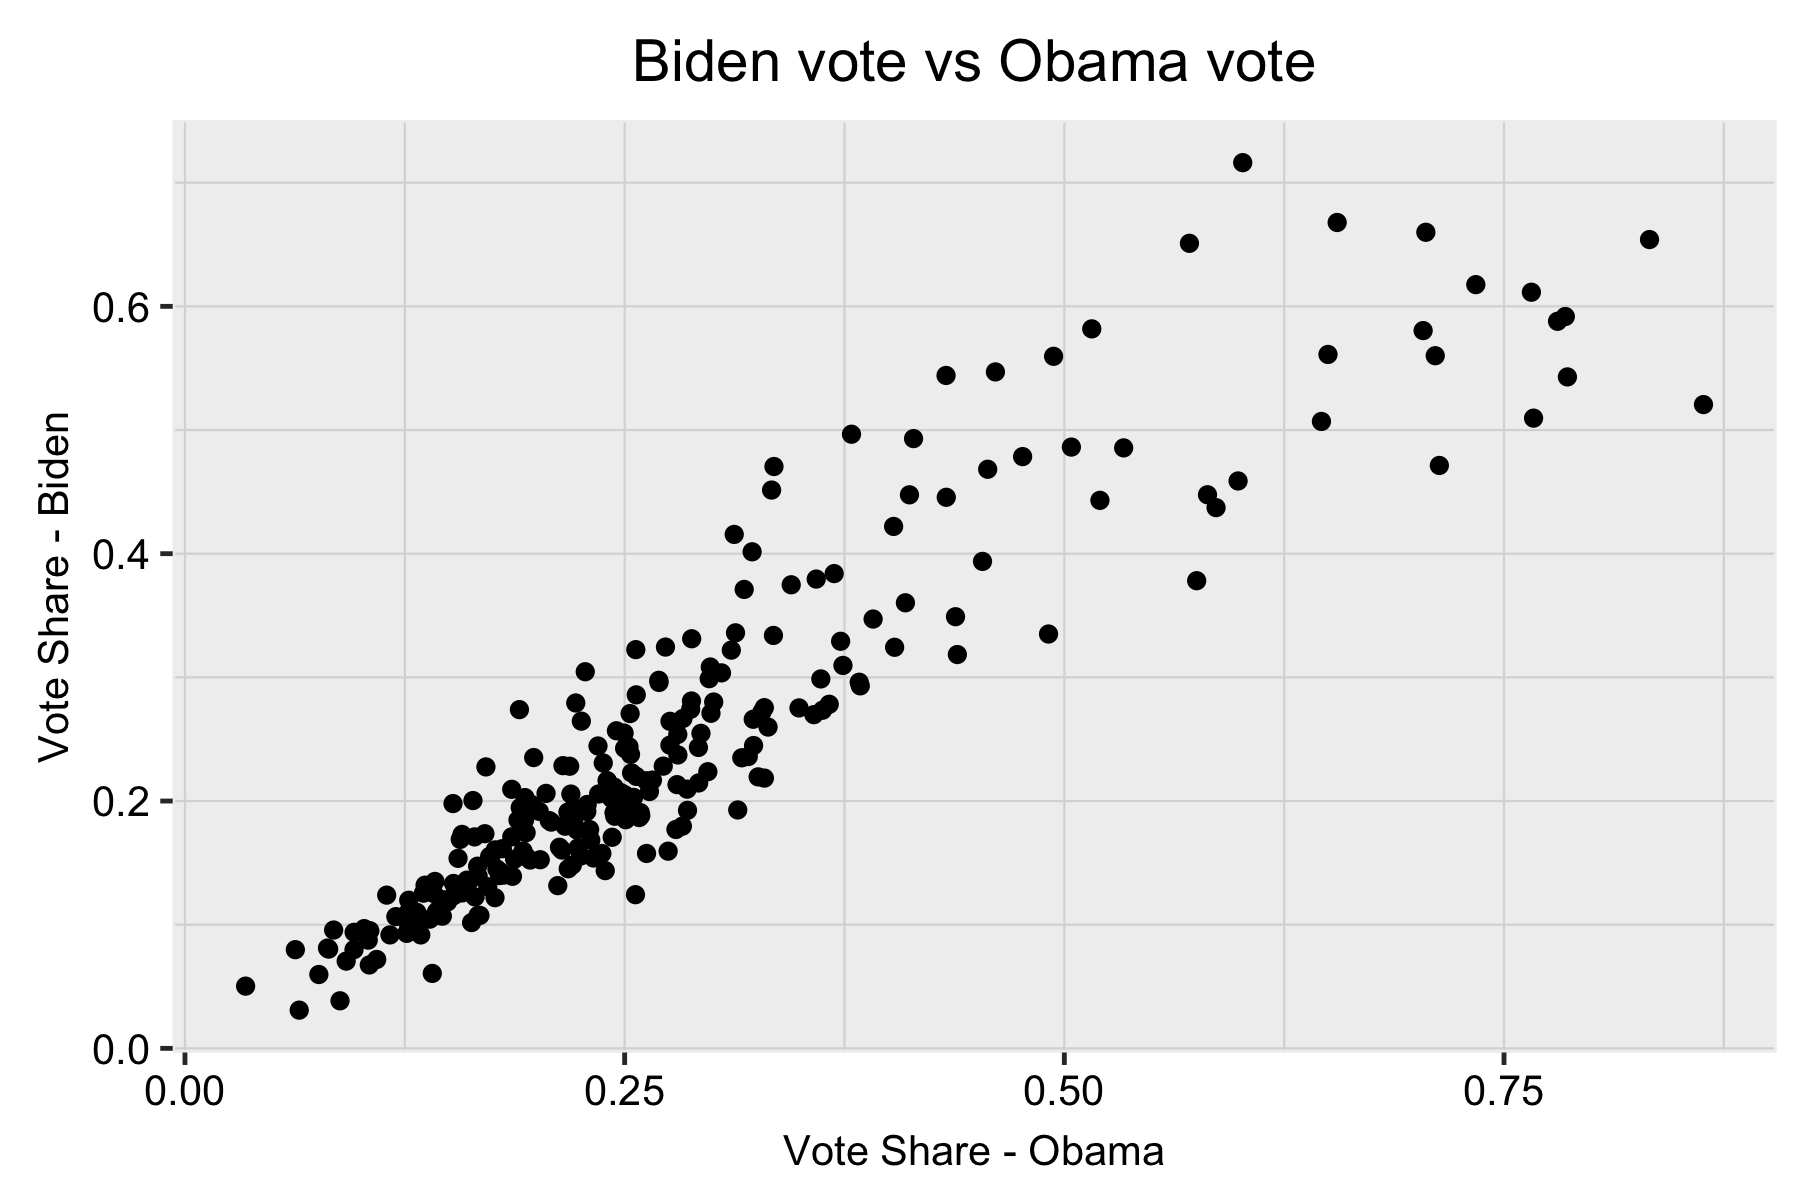
\includegraphics[width = 0.7 \linewidth]{biden-obama}
		\end{center}
		\begin{wideitemize}
		\item
		If we look at the data, we see that Biden vote share is highly positively correlated with Obama vote share.
		
		\item
		So what's going on?!
	\end{wideitemize}
	\end{frame}
	
	\begin{frame}{Interpreting Regression Coefficients}
		\begin{wideitemize}
			\item
			Remember that multivariate OLS is approximating the CEF as
			$$E[Y_i | \bm{X}_i = \bm{x}] \approx \beta_0 +  x_{i1} \beta_1 + x_{i2} \beta_2 $$
			
			\pause
			\item
			Thus, $\beta_2$ is an estimate of a \textit{partial derivative},
			
			$$\dfrac{\partial }{\partial x_{i2}}  E[Y_i | \bm{X}_i = \bm{x}] \approx \beta_2 ,$$
			
			\noindent i.e. the change in the CEF from changing $X_{i2}$ \textit{holding $X_{i1}$ constant}. 
			
			\pause
			\item
			If $\beta_2 < 0$, this means that among places where Clinton had the same vote share, Biden did better in places with lower Obama vote share.
			
			\pause
			\item
			In other words, Biden did better in places where Democratic vote share was increasing between 2012 and 2016!
		\end{wideitemize}	
	\end{frame}

	\begin{frame}
		\centering
		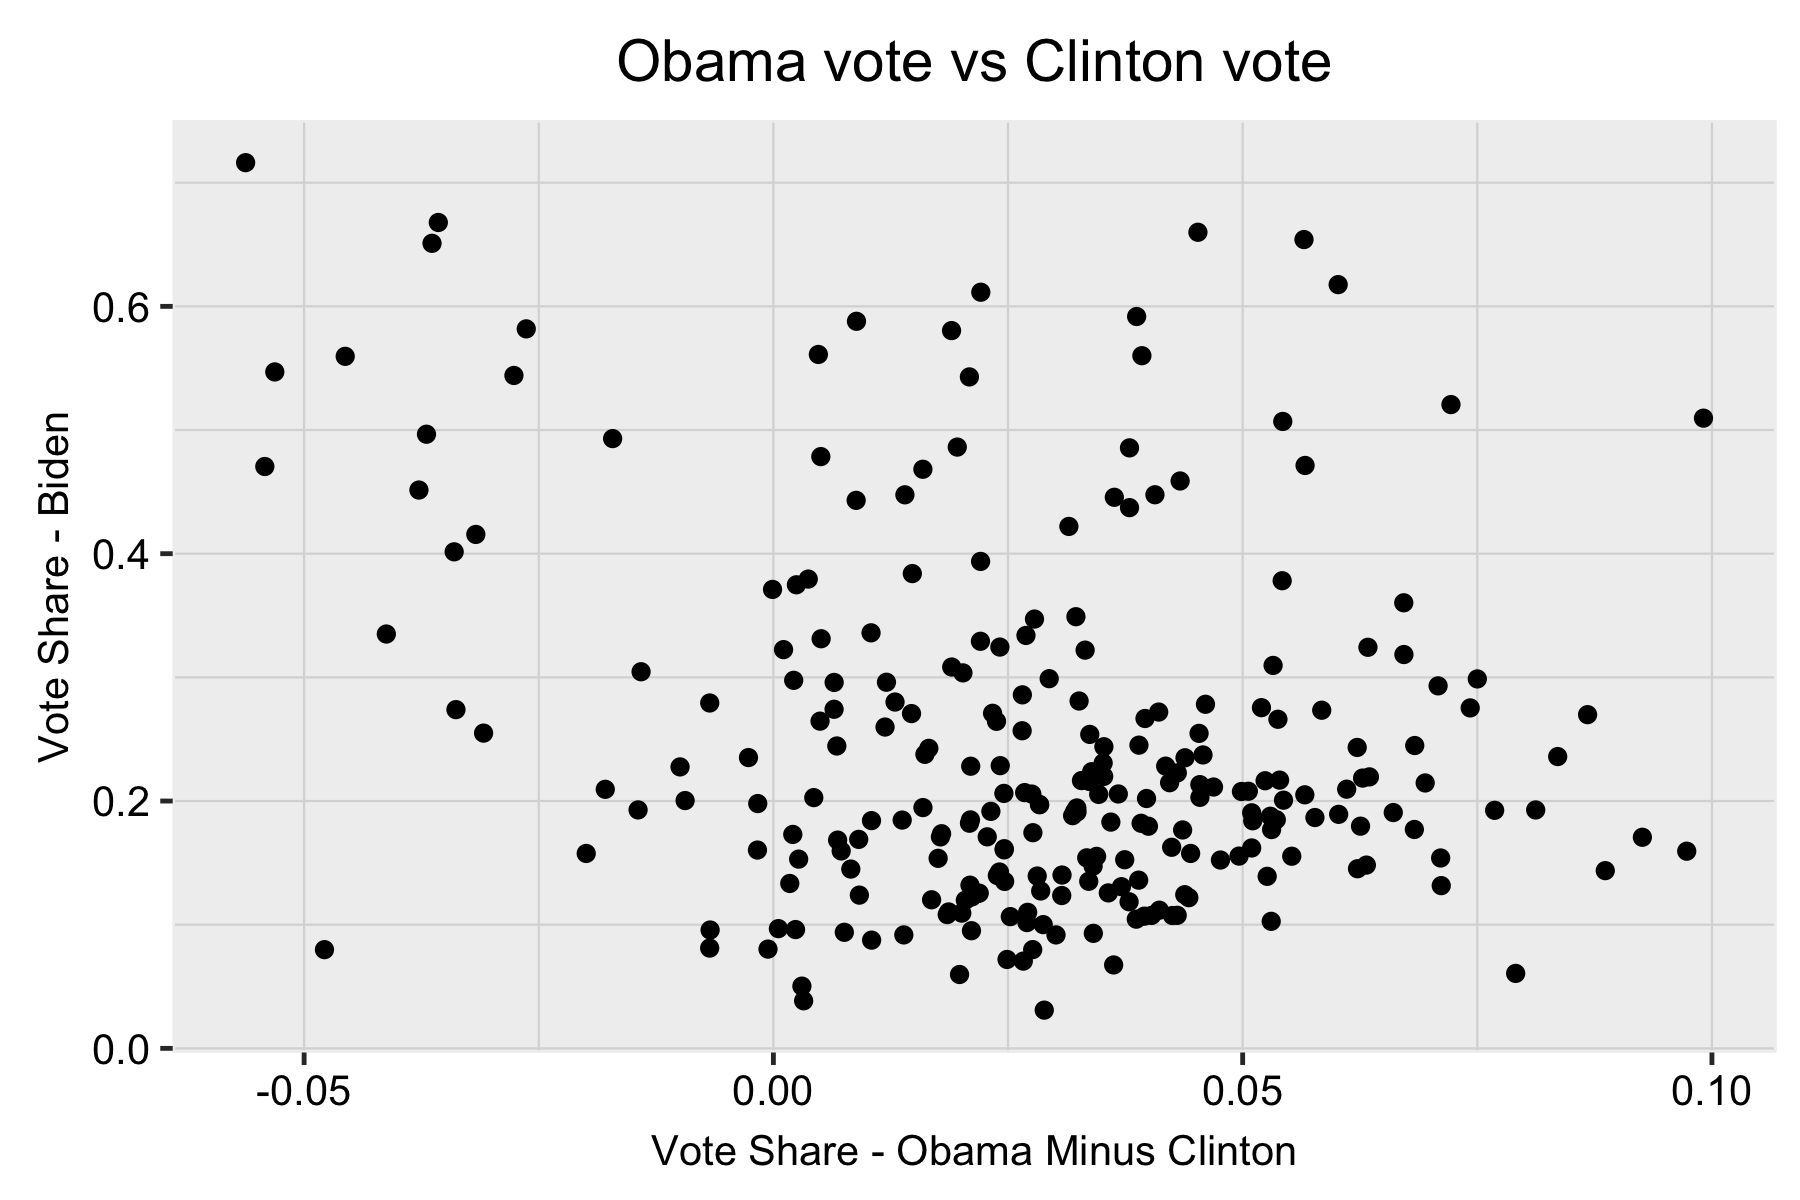
\includegraphics[width = 0.8 \linewidth]{biden-obama-minus-clinton}
	\end{frame}


	\begin{frame}{Generalizing this idea}
		\begin{wideitemize}
			\item
			The \textbf{Frisch-Waugh-Lovell} (FWL) theorem gives us a general way to interpret coefficients in multivariate regression. \pause Consider the regression
			$$Y_i = \beta_0 + X_{i1} \beta_1 + X_{i2} \beta_2 + \epsilon_i$$
			
			
			\pause
			\item
			FWL says that the OLS coefficient $\hat\beta_2$ can be obtained by the following steps:
			
			\pause
			\item
			1) Regress $X_{i2}$ on $X_{i1}$ and a constant:
			$$X_{i2} = \gamma_0 + X_{i1} \gamma_1 + u_i $$
			
			\pause
			\item
			2) For each unit, predict $X_{i2}$ using the coefficients obtained in step 1)
			$$\hat{X}_{i2} = \hat\gamma_0 + X_{i1} \hat\gamma_1 $$
			
			\pause
			\item
			3) Obtain $\hat\beta_2$ by regressing $Y_i$ on the OLS residual $X_{i2} - \hat{X}_{i2}$:
			$$Y_i =  \alpha + (X_{i2} - \hat{X}_{i2})  \beta_2 + v_i$$
			
		\end{wideitemize}		
	\end{frame}

	\begin{frame}{Illustration Using Election Data}
	\begin{wideitemize}
		\item
		Regress Obama vote share on Clinton vote share
		\begin{tabular}{lr}
		Intercept ($\hat\gamma_0$) & 0.03 \\
		Clinton ($\hat\gamma_1$) & 0.98
		\end{tabular}
		
		\pause
		\item
		Predict Obama vote share using Clinton vote share:
		
		$$\hat{X}_{i2} = \pause{} 0.03 + 0.98 X_{i1} $$
		
\vspace{-0.5cm}
		\pause
		\item
		Regress Biden vote share on $X_{i2} - \hat X_{i2} $:
		
		\begin{tabular}{lr}
			Intercept ($\hat\alpha$) & 0.25 \\
			Obama minus predicted ($\hat\beta_2$) & -0.56
		\end{tabular}
	
	\item
	The estimate $\hat\beta_2$, -0.56, is exactly what we got before!				
	\end{wideitemize}	
	\end{frame}
	
	
	\begin{frame}
		\centering
		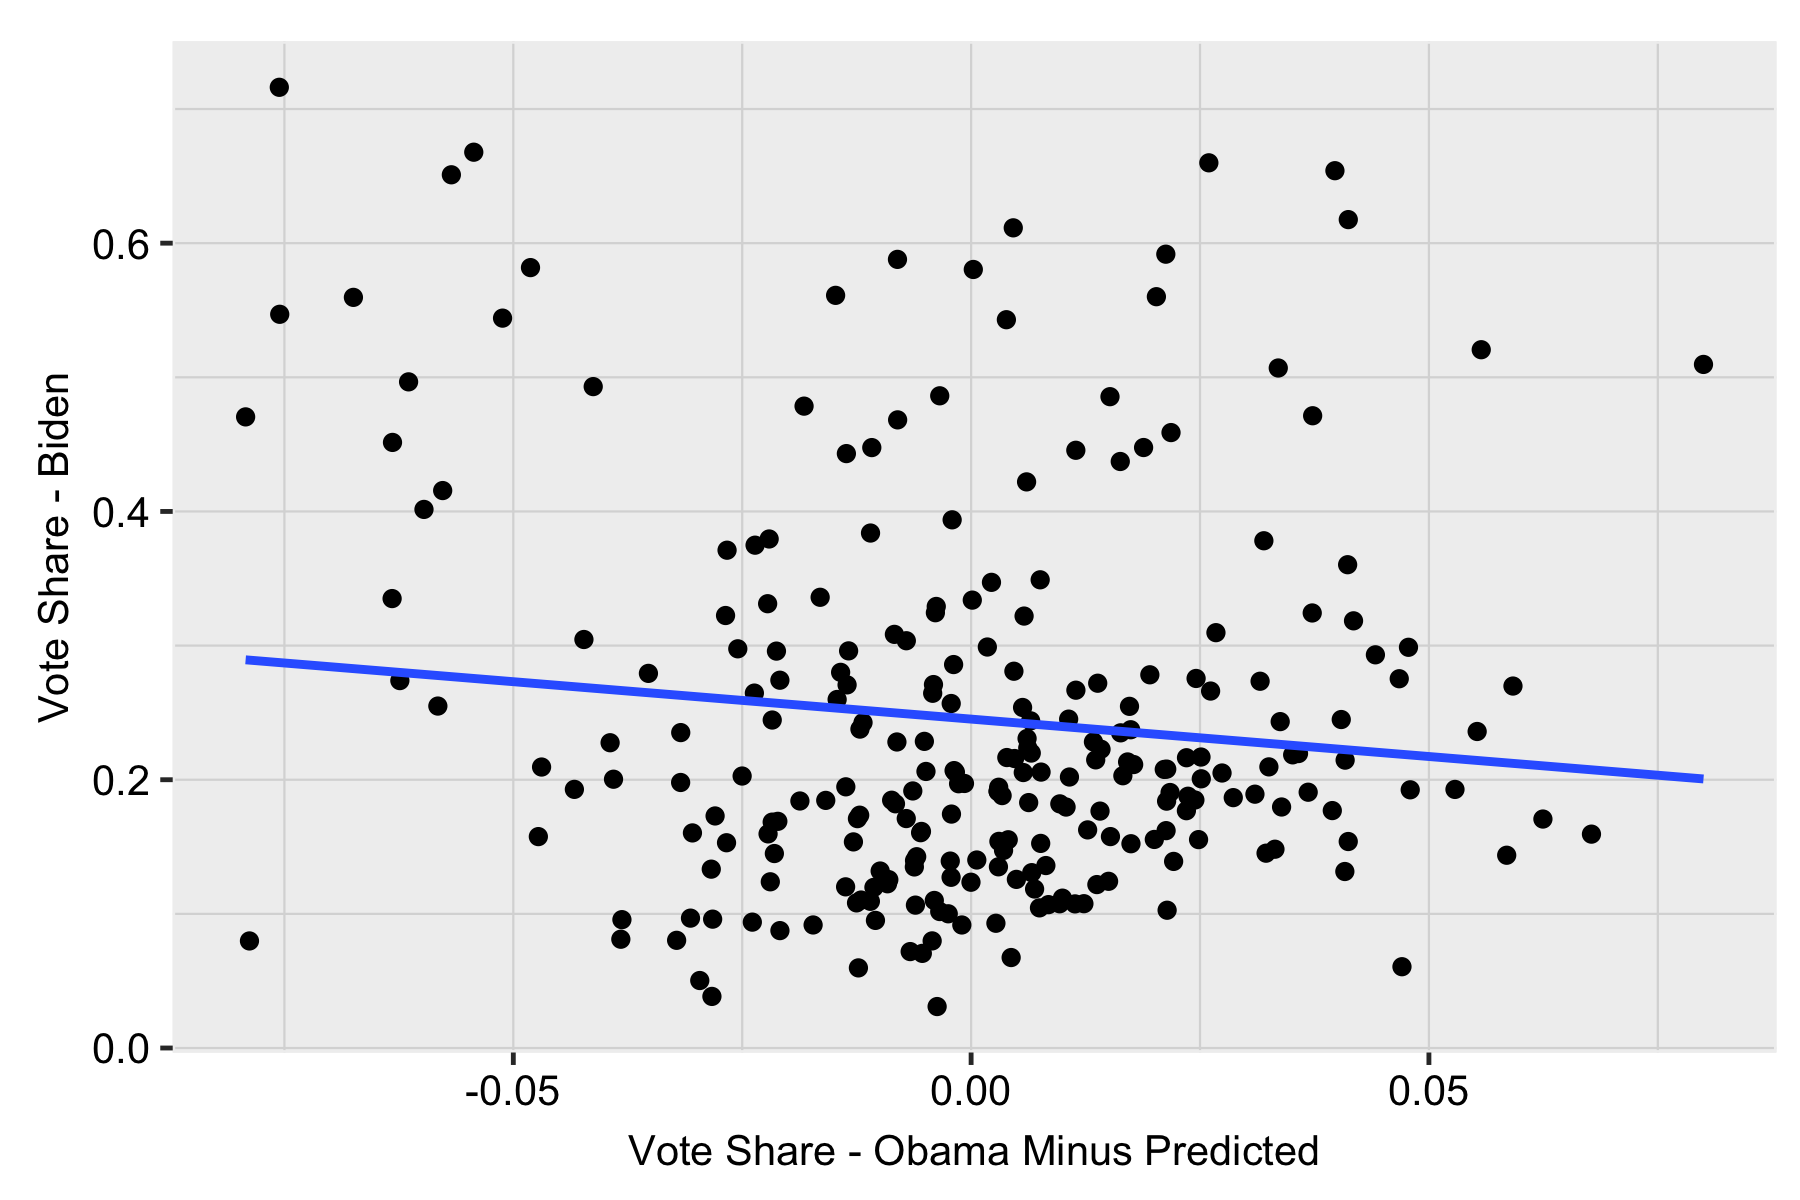
\includegraphics[width = 0.7\linewidth]{biden-obama-residuals}

		\begin{wideitemize}
			\item
			The slope of the best-fit line is precisely $\hat\beta_2 = -0.56$.
			\item FWL generally gives us an easy way to visualize/interpret multivariate regression coefficients 
		\end{wideitemize}
	\end{frame}
	

	\begin{frame}{Measures of Model Fit}
	\begin{wideitemize}
		\item
		Did adding a quadratic term help us improve our approximation to the wage-age CEF? How can we measure this?  
		
		\pause
		\item
		One way of measuring model fit is the population $R^2$: for the regression $Y_i = \bm{X}_i' \bm{\beta} + \epsilon_i$, 
		
		$$ R^2 = \frac{Var(\bm{X}_i' \bm{\beta})}{ Var(Y_i) } $$
		
		\pause
		\item
		Intuitively, population $R^2$ measures the fraction of the variance of $Y_i$ explained by $\bm{X}_i ' \beta$\smallskip
\begin{itemize}
\item Since $Cov(\mathbf{X}_i^\prime\boldsymbol{\beta},e_i)=0$, we also have $R^2=1-\frac{Var(e_i)}{Var(Y_i)}$
\end{itemize}
		
		
		\pause
		\item
		To estimate $R^2$, we replace population values with sample analogs
		
		$$\hat{R}^2 = \frac{\frac{1}{N}\sum_i(\mathbf{X}_i^\prime\hat{\boldsymbol{\beta}}-\bar{\mathbf{X}}_i^\prime\hat{\boldsymbol{\beta}})^2}{\frac{1}{N} \sum_i (Y_i - \bar{Y})^2 }=1 - \dfrac{  \frac{1}{N} \sum_i \hat\epsilon_i^2 }{ \frac{1}{N} \sum_i (Y_i - \bar{Y})^2 }$$
	\end{wideitemize}
\end{frame}


\begin{frame}{$R^2$ in the Wage-Age Example}
	\begin{figure}
		\subfloat[$\hat{R}^2$ = 0.44]{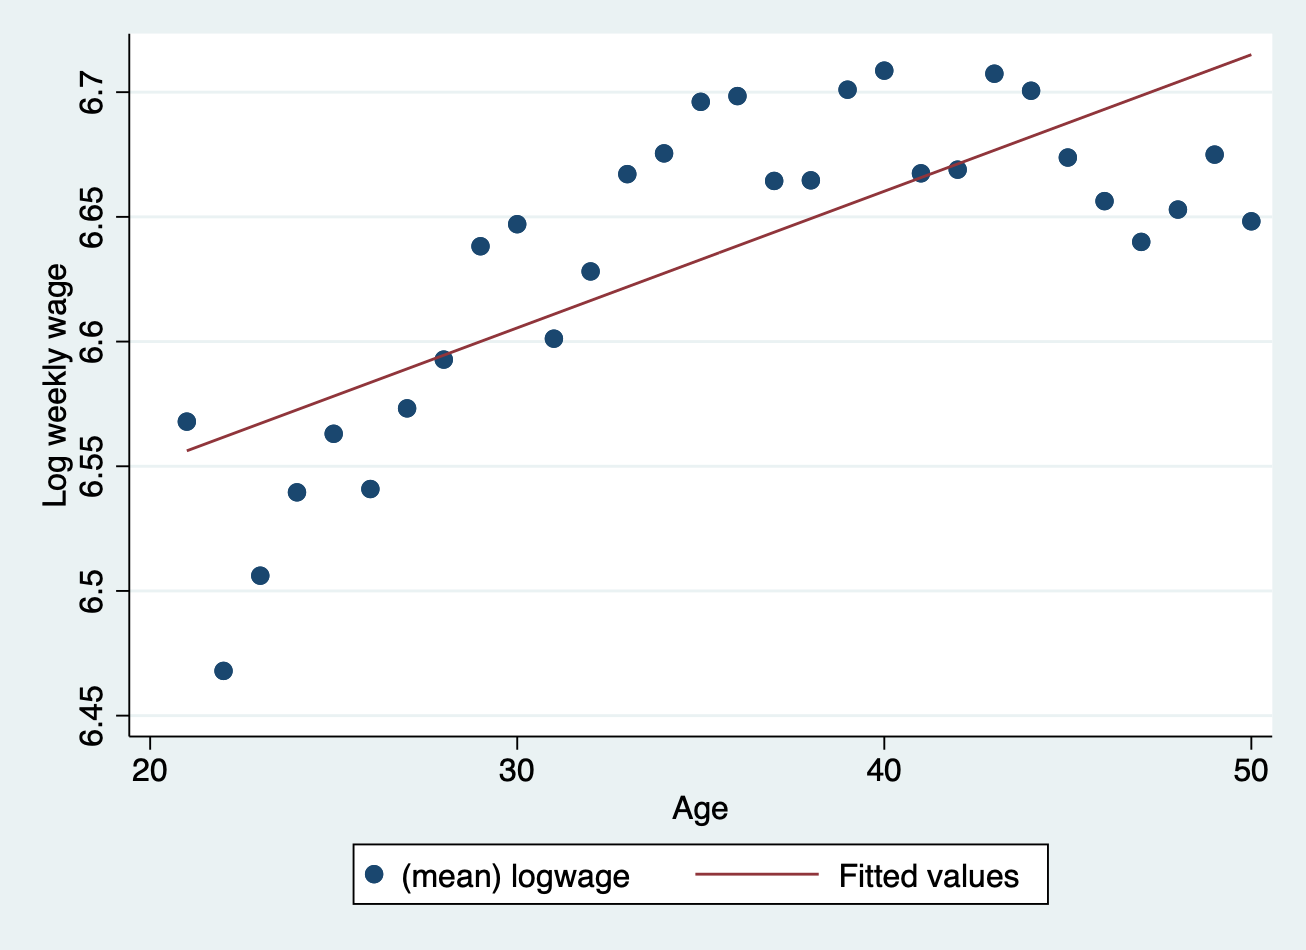
\includegraphics[width = 0.45 \linewidth]{logwages-linear}}  \subfloat[$\hat{R}^2$ = 0.73]{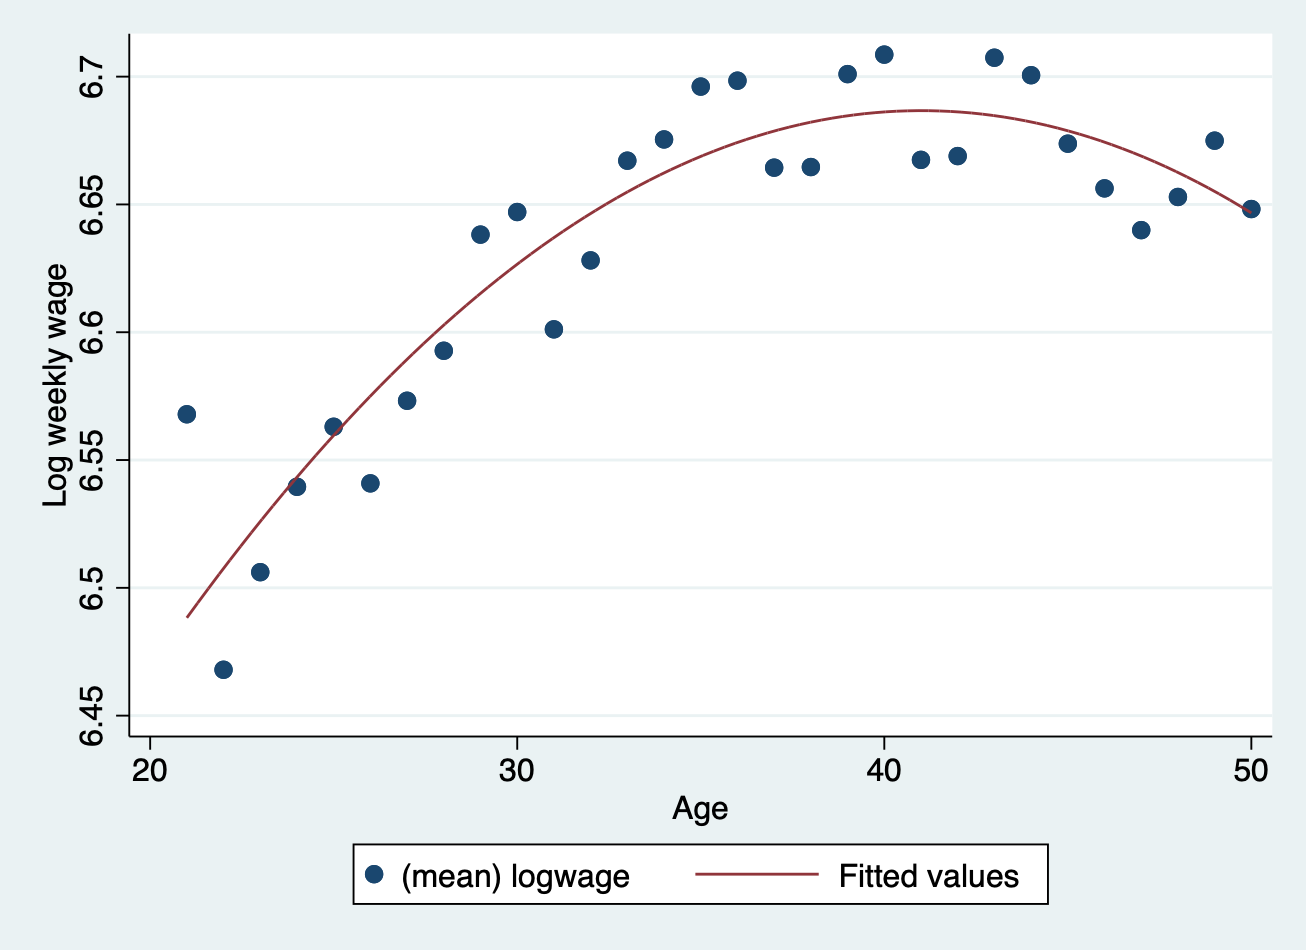
\includegraphics[width = 0.45 \linewidth]{logwages-quadratic}}
	\end{figure}
	
	\begin{wideitemize}
		\item
		The linear fit explains 44\% of the variation in average earnings across ages, whereas the quadratic fit explains 73\%
	\end{wideitemize}
\end{frame}


\begin{frame}{Caution about $\hat{R}^2$}
	\begin{wideitemize}
		\item
		Caution: the sample $\hat{R}^2$ will always increase if you have a more complicated model. Why? 
		
		\pause
		\item
		The coefficients from a linear fit minimizes 
		$$ \frac{1}{N} \sum_i (\underbrace{Y_i - (\hat\beta_0 + \hat\beta_1 X_i)}_{\hat\epsilon_{Linear}})^2 $$
		
		While the coefficients in a quadratic fit minimize
		
		$$ \frac{1}{N} \sum_i (\underbrace{Y_i - (\hat\beta_0 + \hat\beta_1 X_i + \hat\beta_2 X_i^2)}_{\hat\epsilon_{Quad}})^2 $$
		
		\noindent Since $\hat\beta_2 = 0$ is feasible in the quadratic minimization, the minimization will always be weakly lower w/a quadratic term
		
		
		\pause
		\item
		But is a more complicated model always better?
	\end{wideitemize}
\end{frame}

\begin{frame}
	
	\begin{figure}
		\subfloat[Quadratic, $\hat{R}^2$ = 0.44]{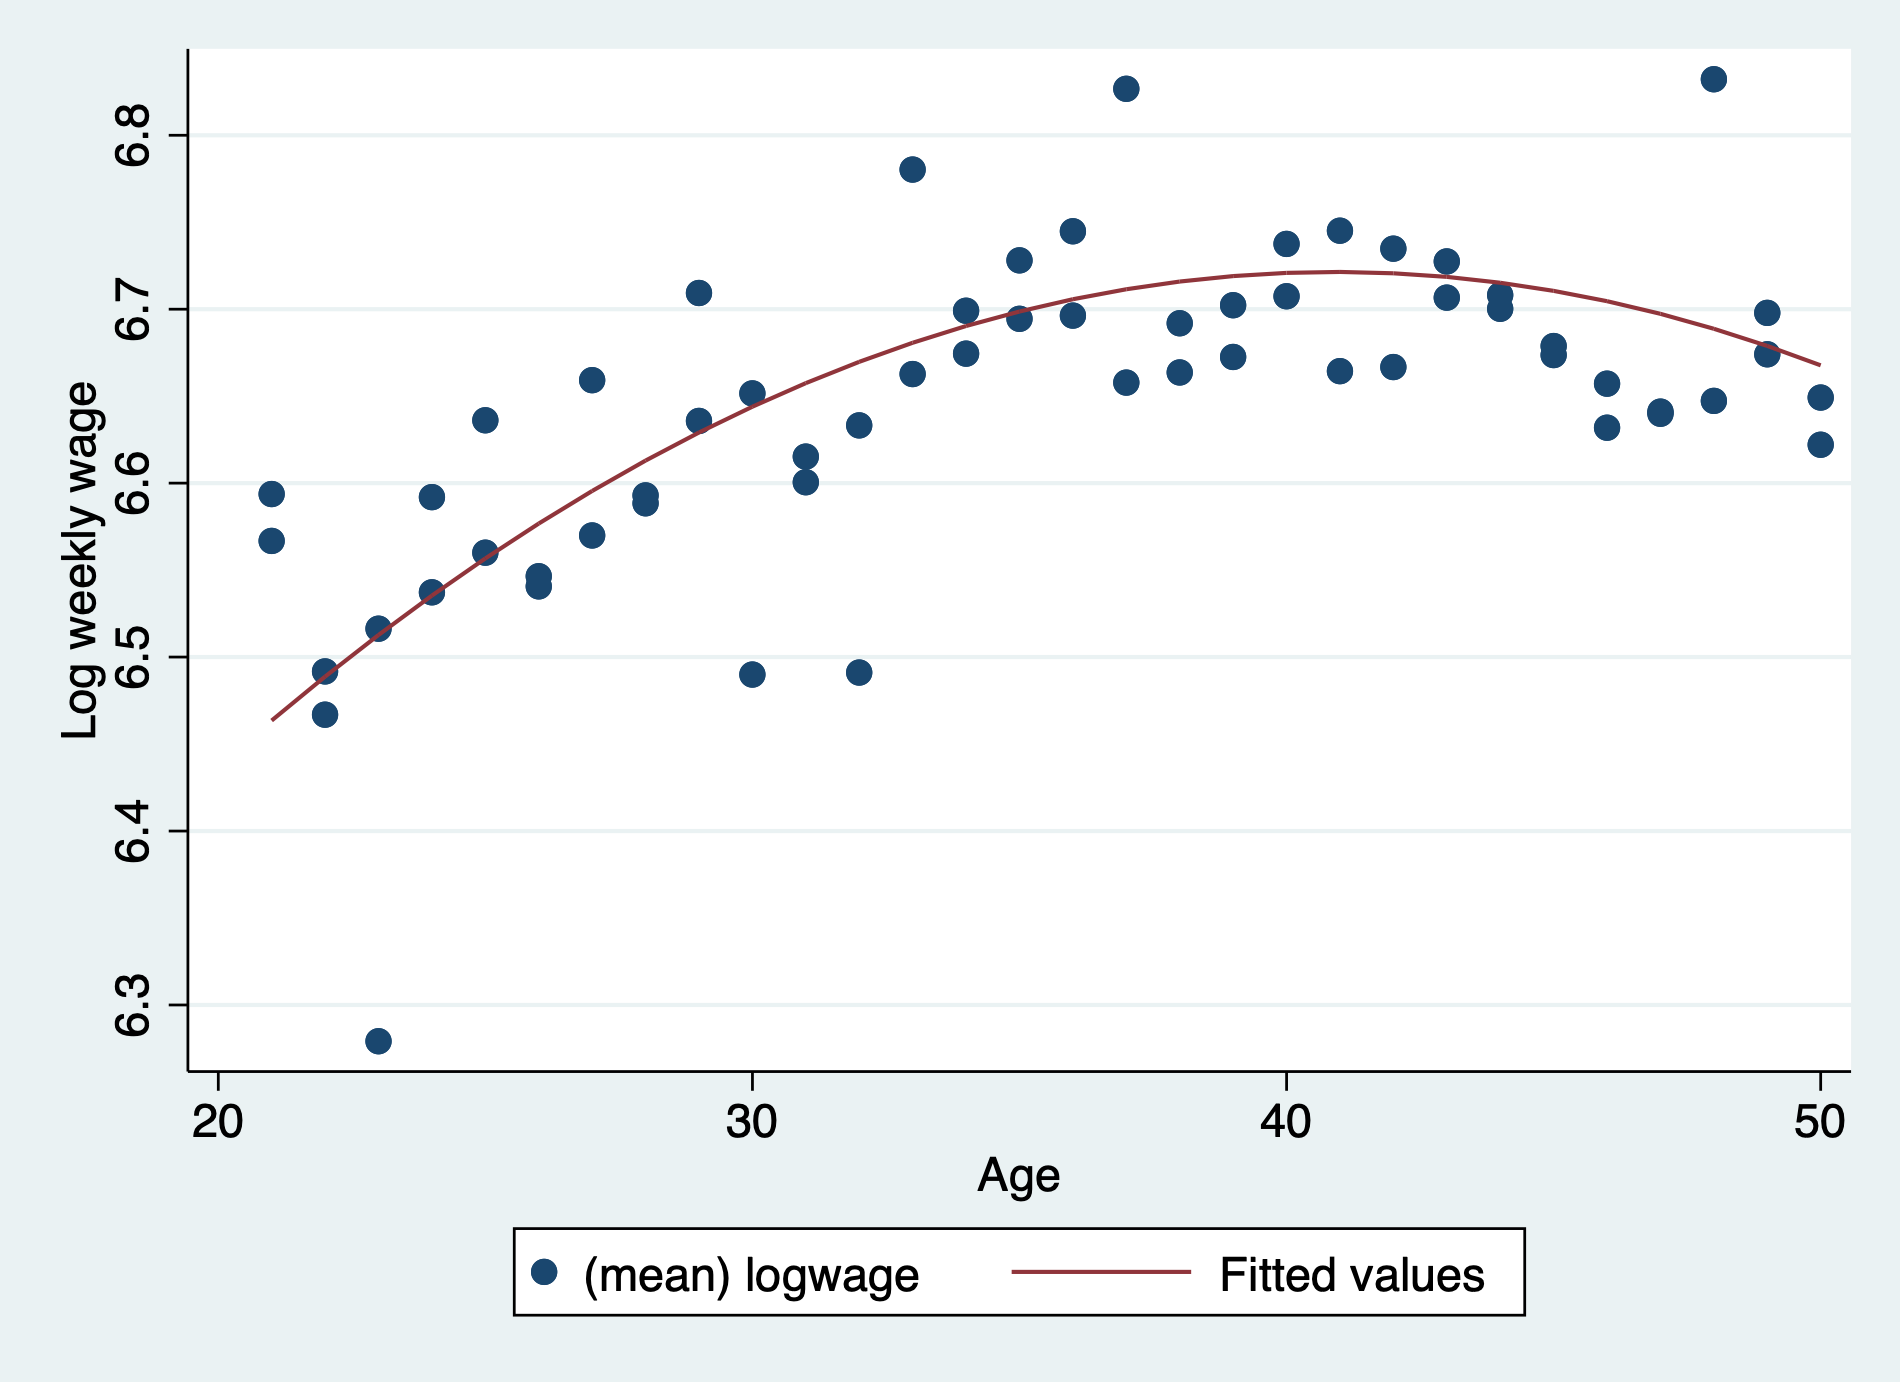
\includegraphics[width = 0.45 \linewidth]{quadfit-insample}}  \subfloat[20th order poly, $\hat{R}^2$ = 0.70]{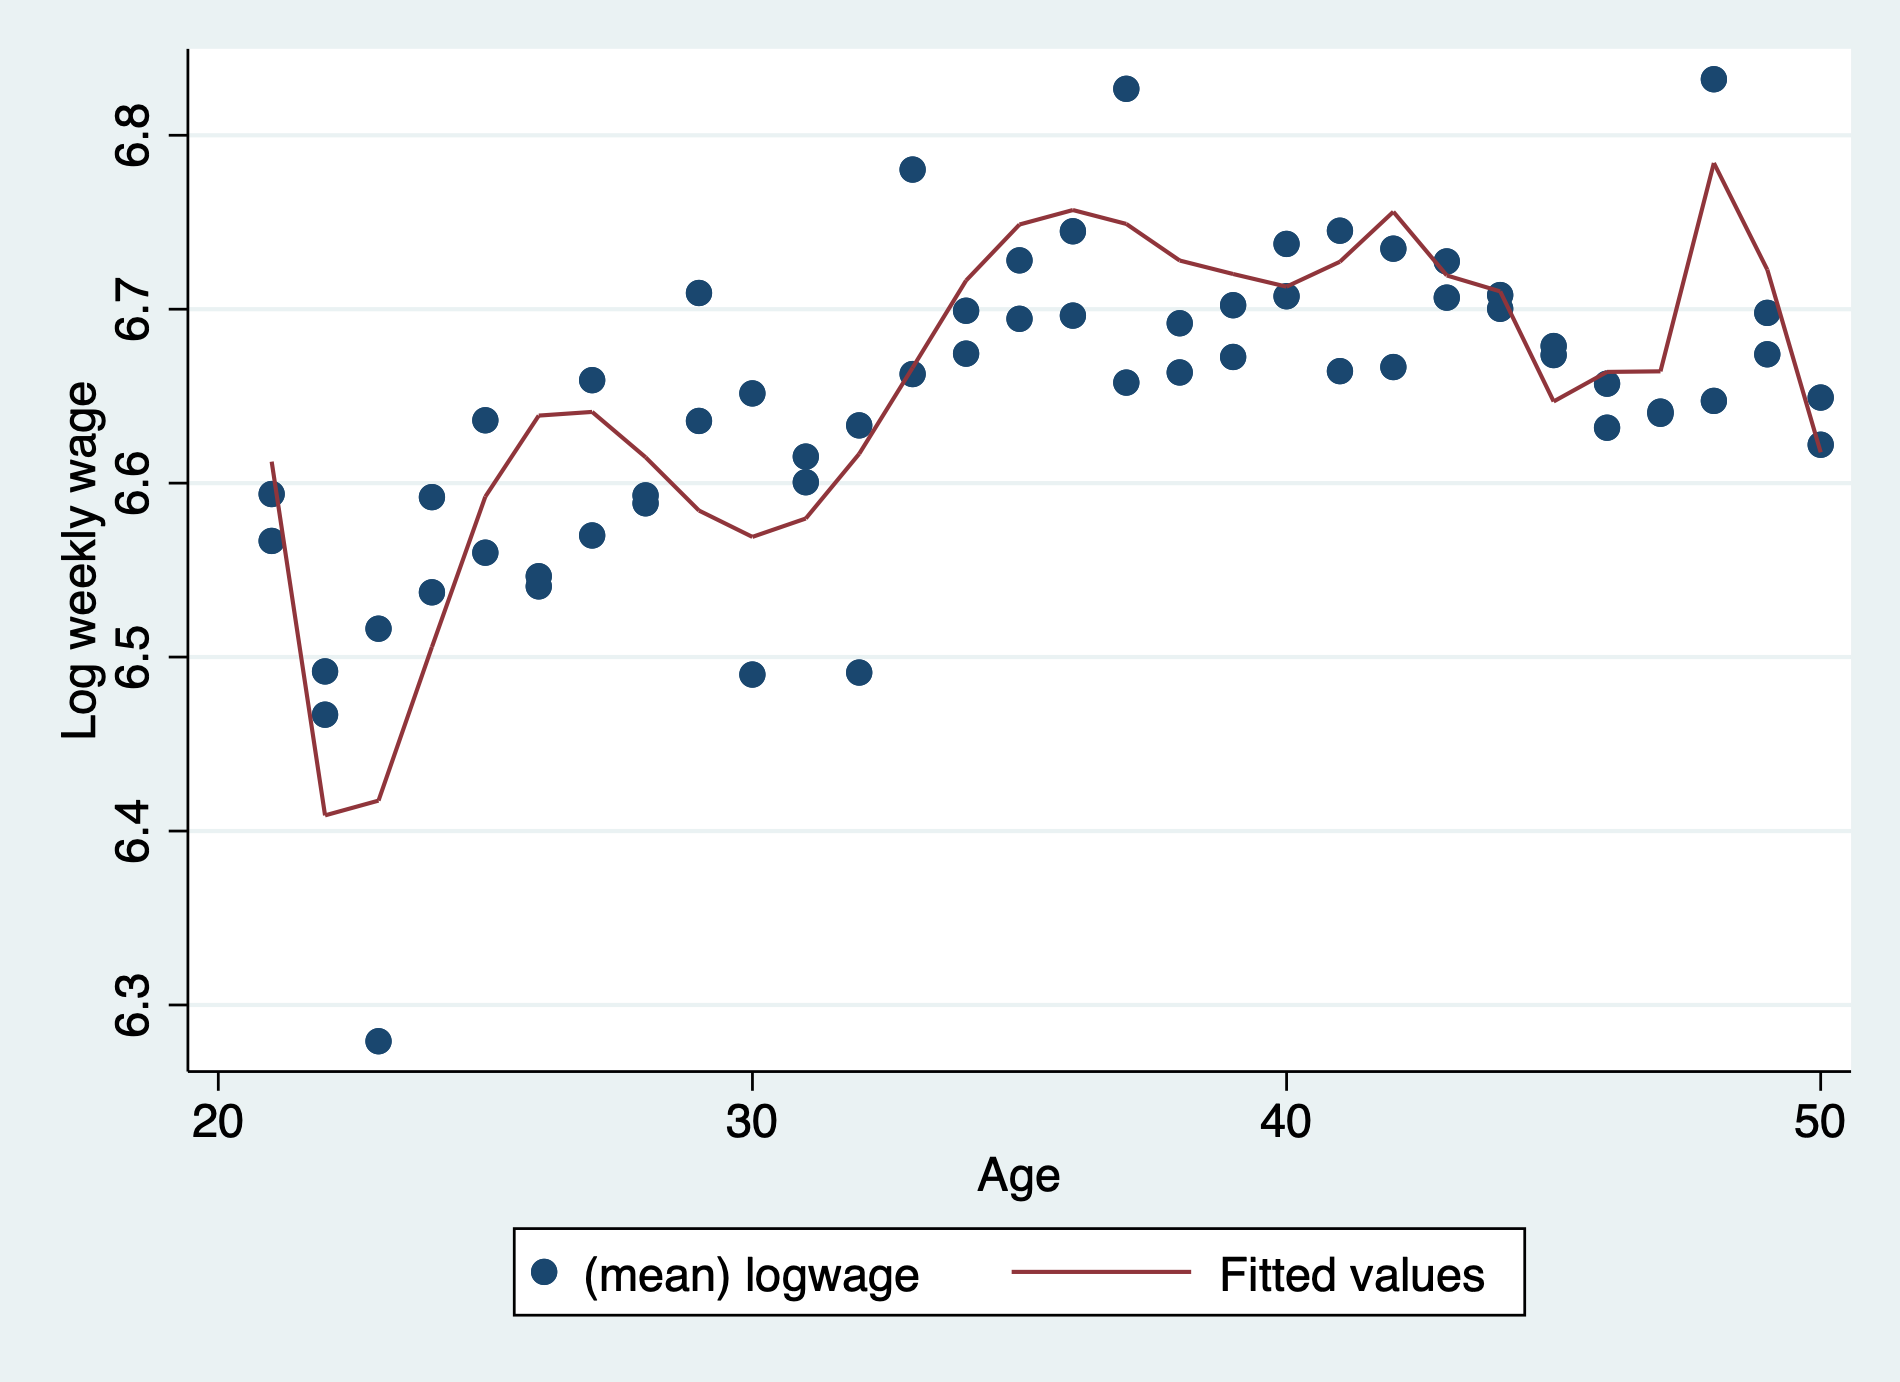
\includegraphics[width = 0.45 \linewidth]{p20fit-insample}}
	\end{figure}
	
	\begin{wideitemize}
		\item
		Suppose we take a sample of size 10,000 and fit a quadratic and a 20th order polynomial
		
		\pause
		\item
		The 20th order poly has higher $R^2$, does it look reasonable to you? 
		
		\pause
		\item
		No, it looks too ``squiggly'' -- it has adapted to fit the exact points in the sample
	\end{wideitemize}
\end{frame}

\begin{frame}
	
	
	\only<2->{ \begin{figure}
			\subfloat[Quadratic]{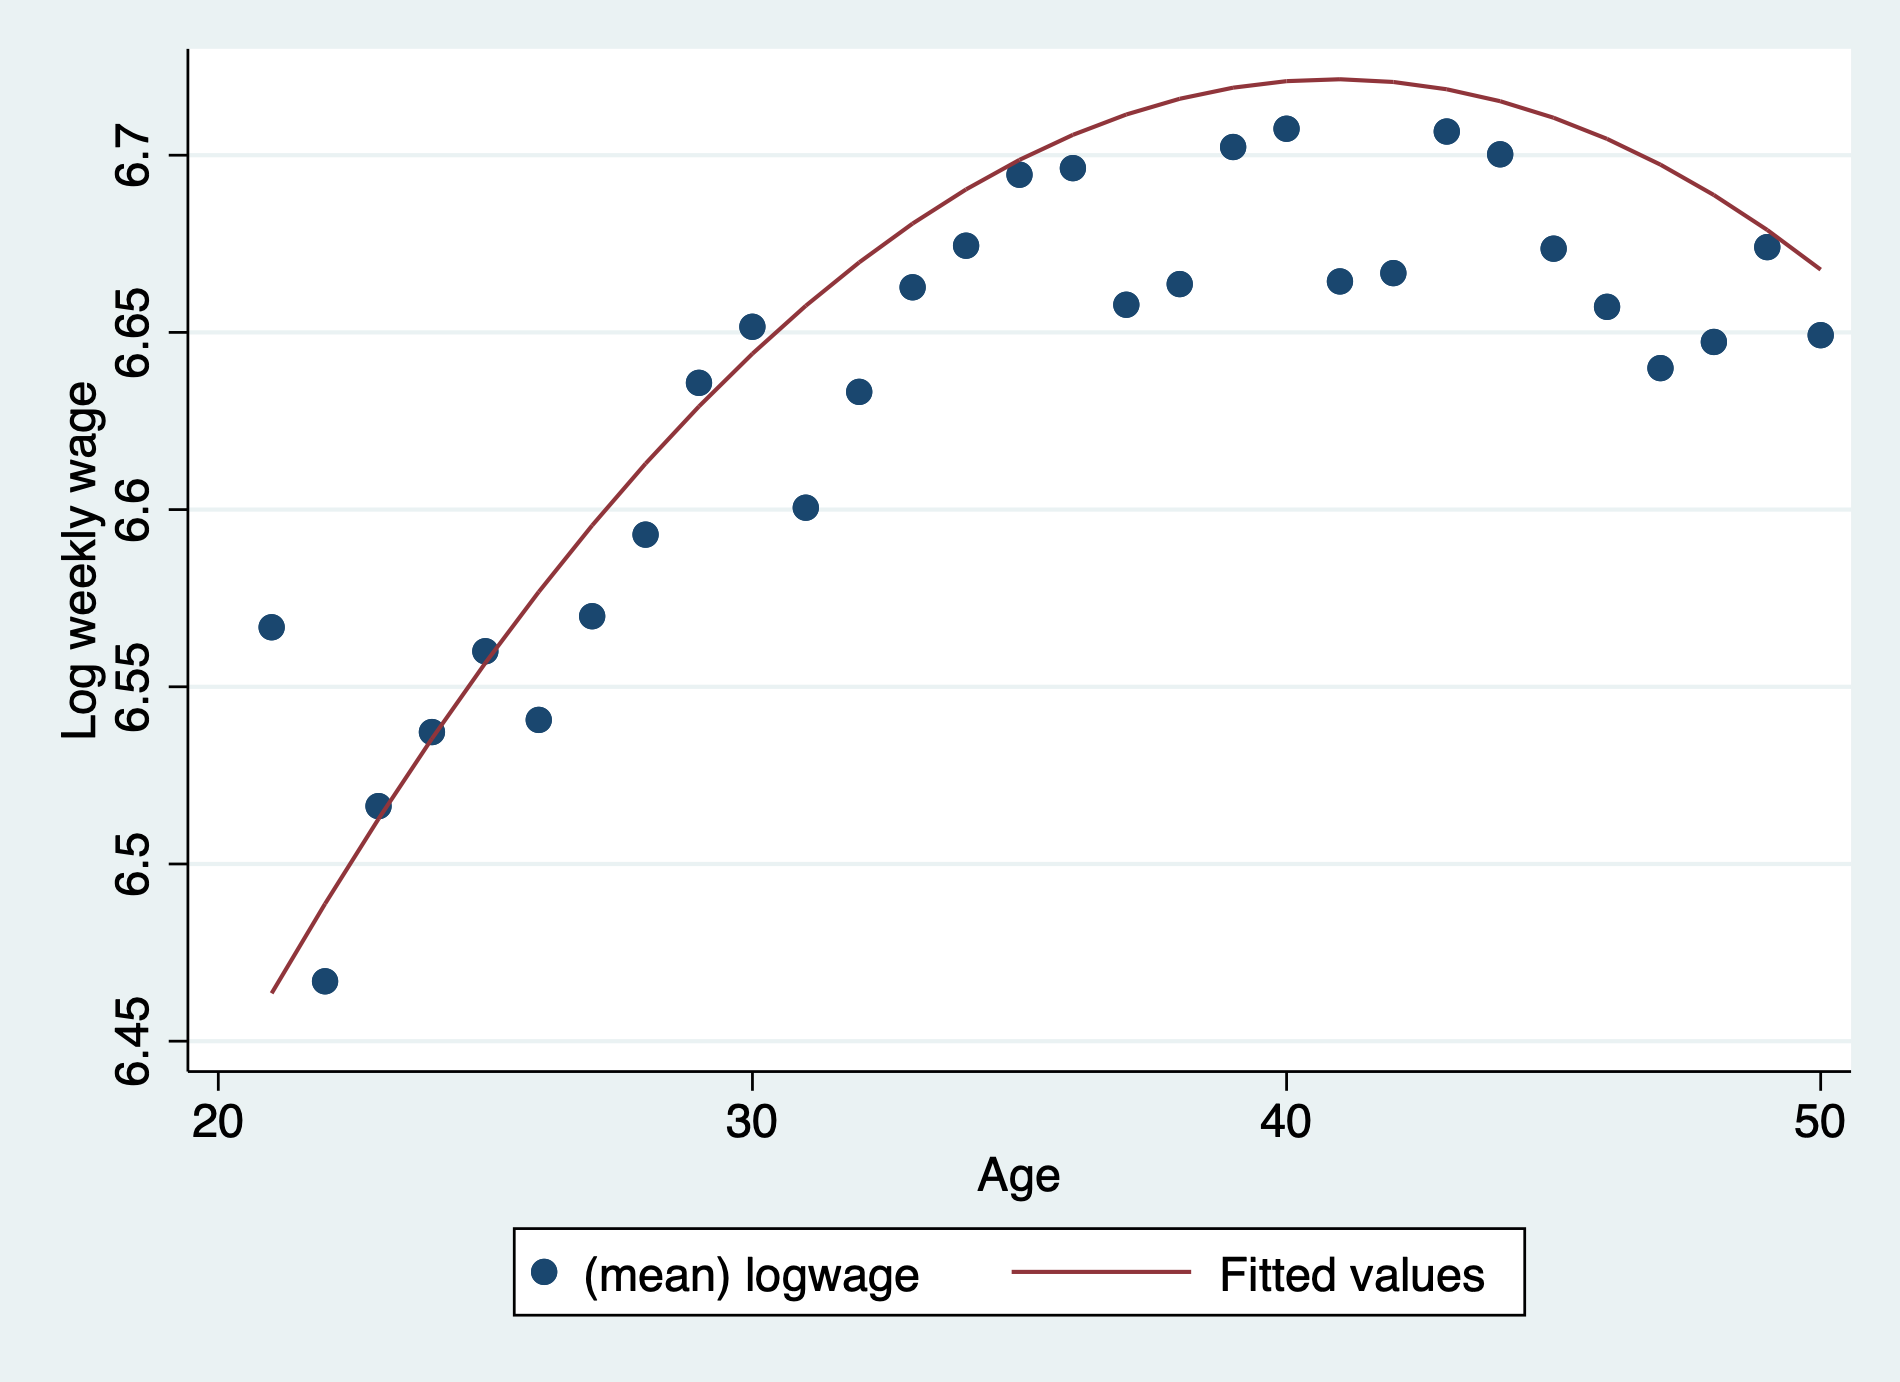
\includegraphics[width = 0.45 \linewidth]{quadfit-outsample}}  \subfloat[20th order poly]{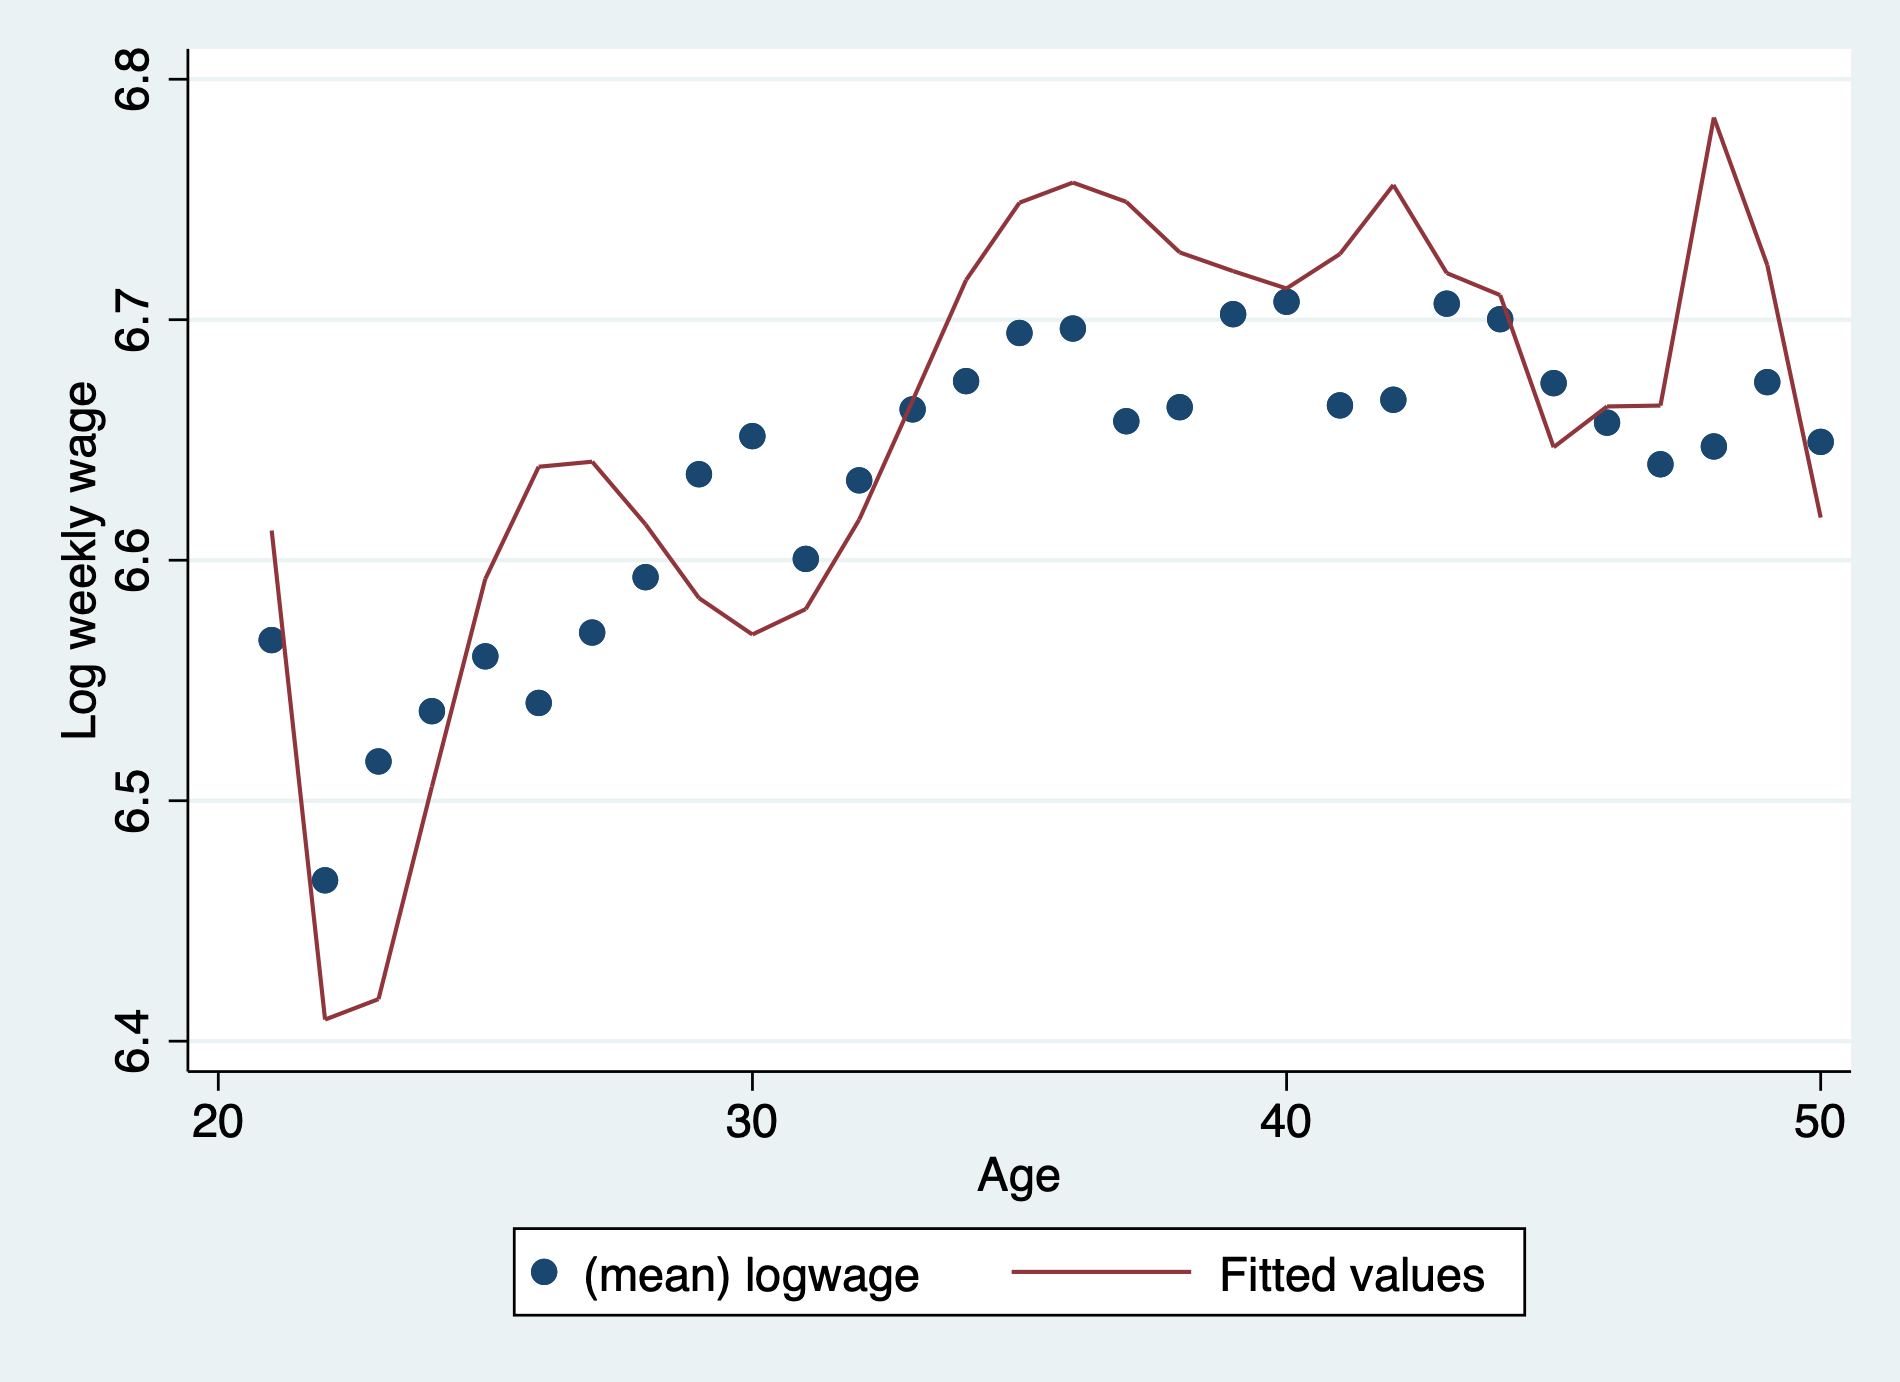
\includegraphics[width = 0.45 \linewidth]{p20fit-outsample}}  		\end{figure}	 }
	
	\begin{wideitemize}
		\item<1->
		Suppose we draw a new sample and test the prediction of our model trained on the first data-set
		
		\pause
		\item
		The quadratic fit generalizes pretty well to the new data.
		
		\item
		But the 20th-order polynomial does very poorly. It ``overfit'' the features of the specific previous sample. This doesn't generalize well to a new sample
		
	\end{wideitemize}
\end{frame}	

\begin{frame}{How Can We Avoid Over-Fitting?}
	\begin{wideitemize}
		
		\item
		The challenge is to pick a rich enough model to capture the key features of the CEF, but not too rich a model such that we overfit
		
		\pause
		\item
		There are several tools available to try to help with this task, none of which is perfect. 
		
		\pause
		\item
		\textbf{Adjusted} $\hat{R}^2$ is a modification to $\hat{R}^2$ that adds a penalty for models with more variables
		\begin{itemize}
			\item
			Generally better than $\hat{R}^2$, but model w/highest $\hat{R}^2$ need not be best
		\end{itemize}	
		
		\pause
		\item
		\textbf{Cross validation}: choose complexity of the model based on how well it does ``out of sample'' \pause
		\begin{itemize}
			\item 
			Split data in two: train model on one half, and see how well it predicts on the second half
			
			\item
			Choose the complexity of the model based on how well it predicts out of sample
			
			\pause
			\item
			Cross-validation is the basis of modern \textit{machine learning} (ML) methods. \\
			ML is very powerful, but how to use ML for causal inference is still being worked out
		\end{itemize}
		
	\end{wideitemize}		
\end{frame}	

\begin{frame}{Avoiding Overfitting in Practice}
	\begin{wideitemize}
		\item
		The tools described above are useful for deciding between models, but in practice model selection is often done more heuristically
		
		\pause
		\item
		Researchers will typically start with a simple model (e.g. linear or quadratic) that includes what they think are the most important variables
		
		\pause
		\item
		Then, they will assess the ``robustness'' of the conclusions to adding/subtracting variables and/or higher-order terms. 
		
		\pause
		\item
		Generally, we will be more confident if the model conclusions are not sensitive to tweaks in the model specification.

%		\pause
%		\item 
%		Of course this is all about maximizing regression ``fit'' -- a different approach is to derive your regression specification from a theoretically-motivated \textbf{causal} query ...
	\end{wideitemize}	
\end{frame}

	
	\begin{frame}{Outline}

	\textcolor{red!75!green!50!blue!25!gray}{1. Deriving Multivariate Regression and OLS}$\checkmark$
	\vspace{0.8cm}
	
	2. Regression and Causality
	\vspace{0.8cm}
	
	\textcolor{red!75!green!50!blue!25!gray}{3. Regression Odds and Ends}
	
	\end{frame}

	\begin{frame}{Regression Meets Causality} 
	
\vspace{0.2cm}
	\begin{wideitemize}
		\item
		Multivariate regressions are often used to estimate causal effects under conditional unconfoundedness
		
		\pause
		\item
		Recall that under conditional unconfoundedness,
		$$CATE(\bm{x}) = E[ Y_{i}  | D_i =1, \bm{X}_i = \bm{x} ] - E[Y_{i} | D_i =0 , \bm{X}_i =\bm{x}]  $$
		
		\pause
		\item
		Common to approximate the CEF linearly, as 
		$$E[ Y_i | D_i, \bm{X}_i  ] \approx D_i  \beta +  \bm{X}_i' \bm{\gamma} $$ 
		
		\pause
		\item
		Then conditional unconfoundedness implies that $CATE(\bm{x}) \approx \beta$. \smallskip
		\begin{itemize}
		\item Doesn't depend on $\mathbf{x}$, so also have $\beta\approx ATE$
		\end{itemize}
		
		\pause
		\item
		So if we estimate the multivariate regression 
		$$Y_i = D_i \beta + \bm{X}_i' \bm{\gamma} + \epsilon_i,$$
		
		\noindent we can interpret $\bm{\hat\beta}$ as an estimate of the ATE.
	\end{wideitemize}
	
\end{frame}




\begin{frame}{Dale and Krueger} 
		\begin{wideitemize}
			\item
			Dale \& Krueger (as you recall) are interested in the effect of attending a more selective college on earnings\smallskip
			\begin{itemize}
			\item
			They have data on earnings and college application information from the College and Beyond (C\&B) Survey 
			\end{itemize}
			\pause
			\item
			The C\&B survey covers students who attended 30 colleges for the high school class of 1978; it contains important variables:
			
			\pause
			\item
			\textbf{Earnings} in 1996
			
			\item
			\textbf{College application and demographic variables} including SAT scores, class rank, family income, race, etc
			
			\item
			\textbf{College application decisions} --- i.e. the set of schools students applied to and were admitted
				
		\end{wideitemize}	
\end{frame}

\begin{frame}
\centering	
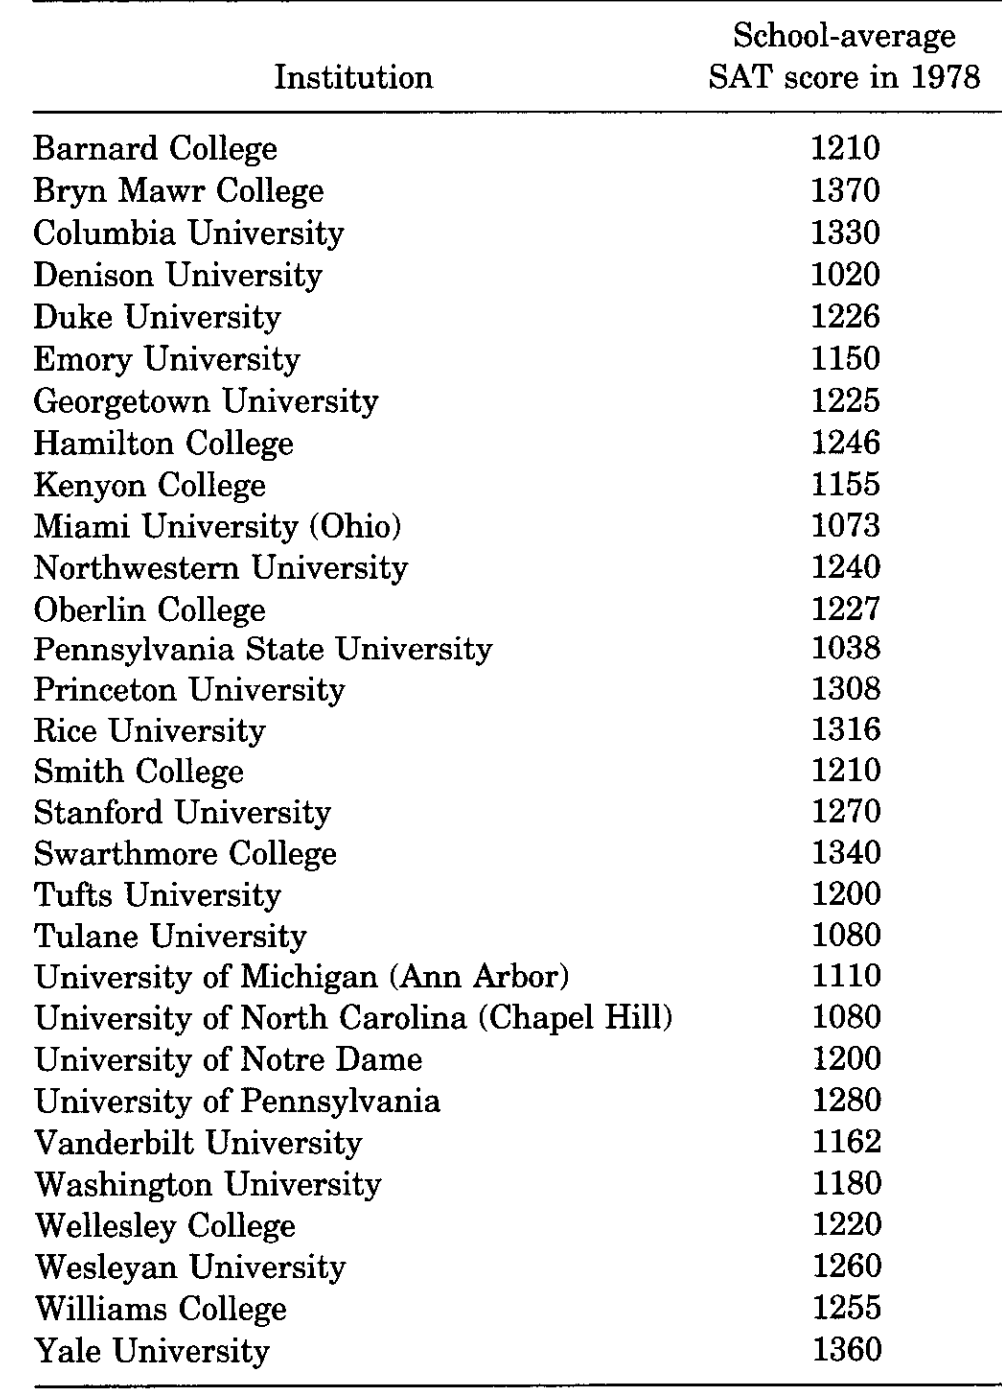
\includegraphics[width = 0.5\linewidth]{dk-list-of-schools}
\end{frame}

\begin{frame}{Dealing with Selection}
	\begin{wideitemize}
		\item
		Dale \& Krueger assume \textbf{conditional unconfoundedness}, i.e. $D_i \indep (Y_i(\cdot)) | X_i$ where $D_i$ is the average SAT score for students at your college and $X_i$ is a set of controls
		
		\pause
		\item
		They then estimate regressions of the form 
		
		$$ln(Y_i) = D_i \beta + \bm{X}_i'\bm{ \gamma }+ \epsilon_i$$
		
		\noindent where $Y_i$ is 1996 earnings
		
		\pause
		\item
		If conditional unconfoundedness holds \& the regression approx. to the CEF is decent, then $\beta$ should (approximately) equal the treatment effect of attending a college with higher average SAT scores.
	\end{wideitemize}
\end{frame}


\begin{frame}{First Pass: SAT Scores and Demographics in $\bm{X}_i$ }
	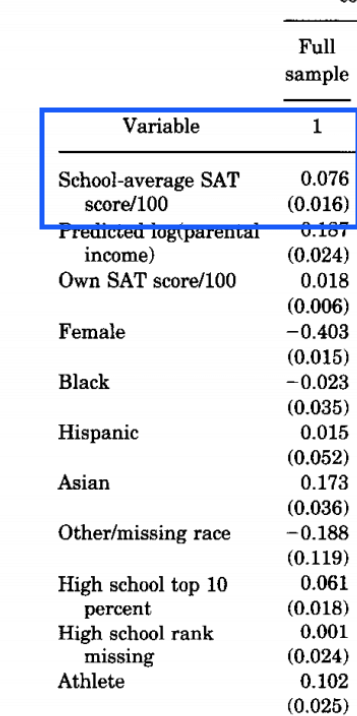
\includegraphics[width =0.3\linewidth]{dk-results-table-reg1}
	
	\begin{wideitemize}
		\item
		$\hat\beta = 0.076$ indicates about an increase in log wages of 7.6 from attending a school with 100 higher SAT points 
	\end{wideitemize}
\end{frame}

\begin{frame}{Do You Buy This Estimate?}
	\begin{wideitemize}
		\item
		Why might unconfoundedness fail when using these controls? \smallskip
			\pause
			\begin{itemize}
				\item 
				Which colleges you get into may depend on relevant unobserved factors --- e.g., students with better application essays may get into more colleges and earn more regardless of where they go
			\end{itemize}
		
		\pause
		\item
		To address this concern, Dale and Kruger have a second analysis: control for the set of colleges that a student applied to / was admitted\smallskip
\pause
			\begin{itemize}
				\item 
				Are able to see this because of the C\&B data
			\end{itemize}
		
		
	\end{wideitemize}
	
\end{frame}


\begin{frame}{Introduction to ``Fixed Effects''}

\begin{wideitemize}
	\item
	What exactly does it mean that they control for the set of colleges you applied / were admitted to?
	
	\pause
	\item
	Consider a simplified version where there are three schools, Brown, Yale, and URI, and everyone applies to all 3. 
	
	
	\pause
	\item
	Suppose all students in the sample get into URI, but admissions decisions at Brown/Yale differ. There are four possible outcomes: \\ \pause
	
	Case 1: Admitted to all schools \\
	Case 2: Admitted to URI and Brown only \\
	Case 3: Admitted to URI and Yale only \\
	Case 4: Admitted to URI only \\
	
	\pause
	\item
	We can construct variables where $X_{i1} = 1$ if we're in case 1 and is 0 otherwise, $X_{i2} = 1$ if we're in case 2 and is 0 otherwise, etc. 
	
	
	\pause
	\item
	The variables $X_{i1},...,X_{i4}$ are often called ``fixed effects'' for the set of schools you were admitted to.
	
	
\end{wideitemize}
\end{frame} 

\begin{frame}{Introduction to ``Fixed Effects''}
	
\begin{wideitemize}
	\item
	We can then approximate the CEF as 
	$$E[Y_i | \bm{X}_i , D_i ] = D_i \beta_D  + X_{i1} \beta_1 + X_{i2} \beta_2 + X_{i3} \beta_3 + X_{i4} \beta_4 $$
	
	\pause
	\item This allows for a different avg outcome depending on which colleges you were admitted to, and the selectivity of your school ($D_i $)
	
	\pause
	\item
	Intuitively, $\beta_D$ represents the average difference from going to an elite school \textit{among} students who got into the same set of schools
\end{wideitemize}	
	
\end{frame}

\begin{frame}
	\centering
	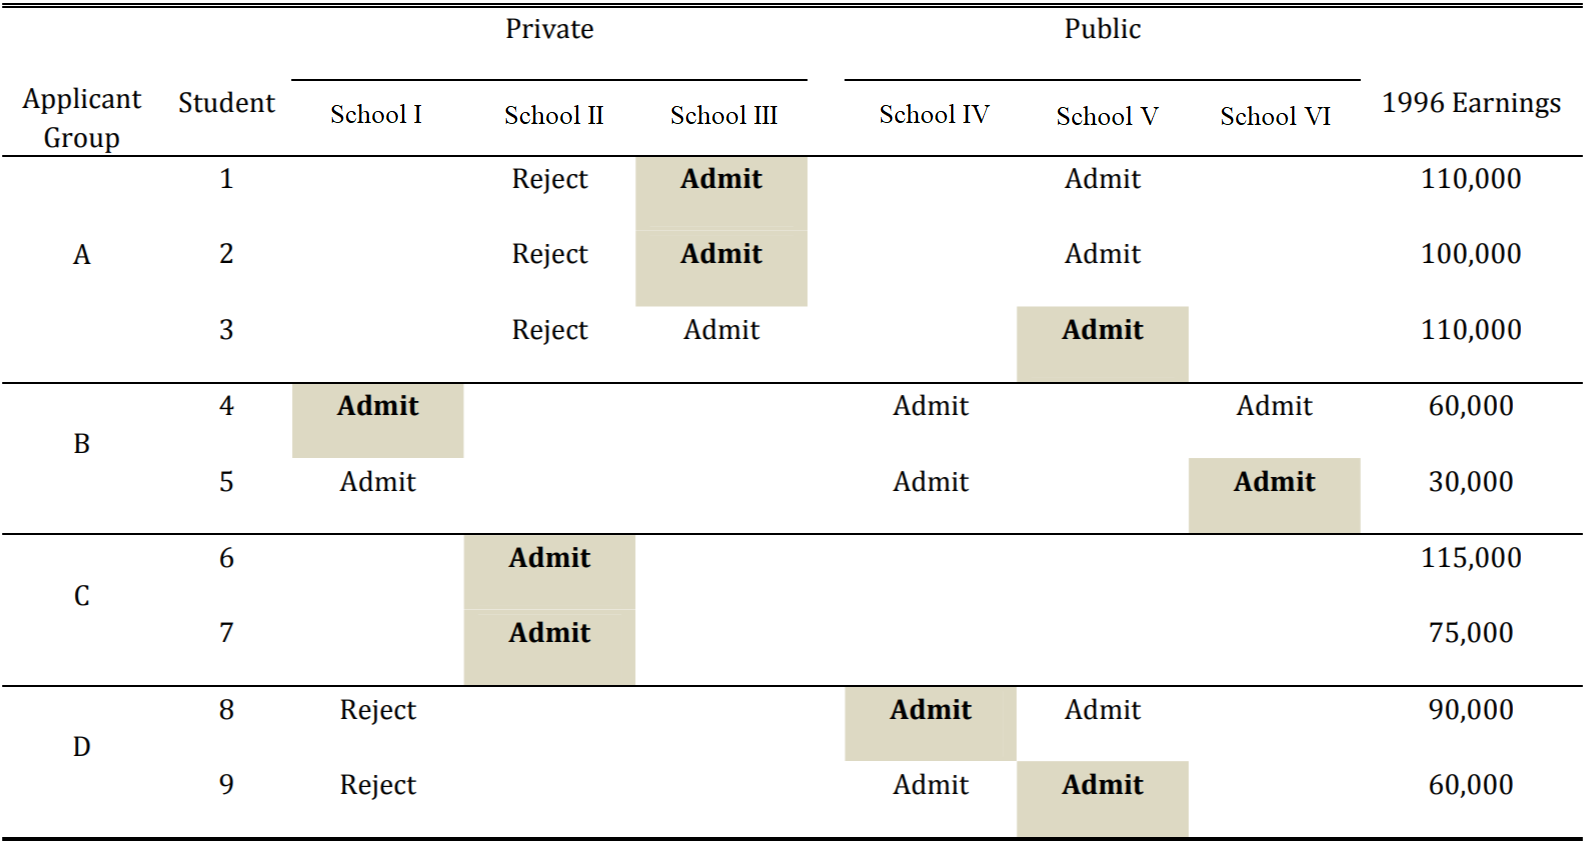
\includegraphics[width = 0.9 \linewidth]{dk-example-applicants}
	\vspace{0.4cm}

	\begin{wideitemize}
		\item
		``Applicant groups'' all applied + admitted to the same set of schools
		
		\item
		The school a student actually attended is highlighted
	\end{wideitemize}
\end{frame}


\begin{frame}{Controlling for Application Decisions in Practice}
	
	
	\begin{wideitemize}
		\item
		In practice, Dale and Krueger don't have that many students who were applied/admitted to the exact same set of schools
		
		\pause
		\item
		As an approximation, they group colleges into bins based on average-SAT rounded to nearest 25 points
		
		\pause
		\item
		They then control for the set of colleges you applied/were admitted to based on these bins (e.g.,  $X_{i1}$ might correspond to being rejected at a school w/SAT 1350 and accepted at 2 schools w/SAT 1250)
		
	\end{wideitemize}
	
\end{frame}

\begin{frame}
	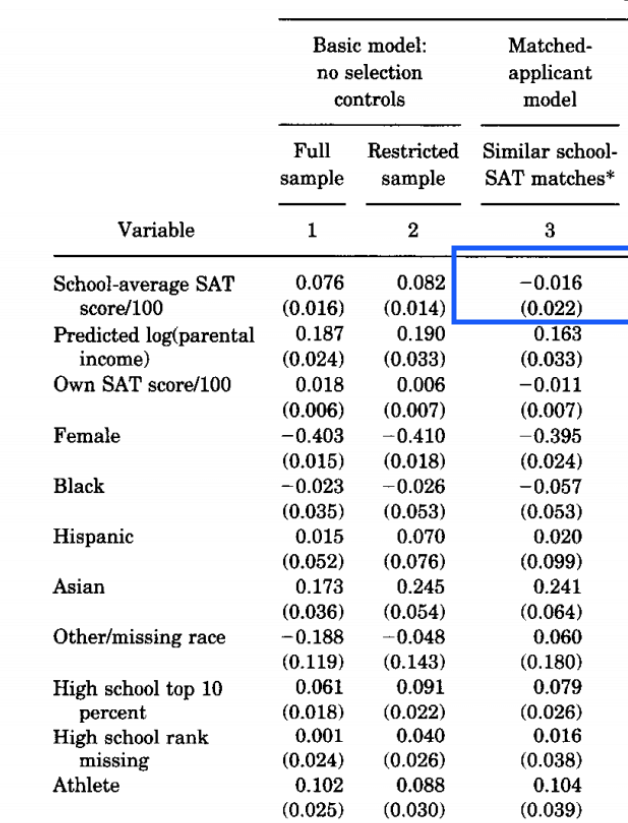
\includegraphics[width =0.5\linewidth]{dk-results-table-reg2}
	
	\begin{wideitemizeshort}
		\item
		With application controls, we get $\hat\beta =-0.016$. 
		
		\pause
		\item
		This indicates about a  -1.6 log wage return to attending a school with 100 higher SAT points (but not significant!)
	\end{wideitemizeshort}
\end{frame}

\begin{frame}{Evaluating Conditional Unconfoundedness (Again)}

\begin{wideitemize}
	\item
	Why might conditional unconfoundedness be violated here? 
	
	\pause
	\item
	A concern is that choice of where to go to college depends on unobservables that are correlated with earnings, even conditional on application choice\smallskip

		\begin{wideitemize}
			\item
			E.g, students who choose to go to a more selective school could have different career ambitions (e.g. industry versus academia)
			
			\pause
			\item
			Students may choose to go to a lower-ranked school only if it has a particularly good program in what they're interested in
			
	 \end{wideitemize}
 
 	\pause
 	\item
 	It's also important to realize that the schools in the C\&B study tend to be selective. These results can at best be interpreted as the causal effect between attending a selective school and highly-selective school
\end{wideitemize}
	
\end{frame}


% PH to here 10/19


\begin{frame}{Omitted Variables Bias}
	\begin{wideitemize}
		\item
		In the C\&B example (and many other applications), we might be worried that we didn't condition on all of the necessary variables for conditional unconfoundedness to hold
		
		\pause
		\item
		How will the coefficients we estimate be biased if we forget to include some variables? 
		
		\pause
		\item
		To answer this question, we will derive what is called the \textbf{omitted variable bias} (OVB) formula
	\end{wideitemize}
\end{frame}


\begin{frame}{Omitted Variable Bias -- Simplest Case}
\begin{wideitemize}
	\item
	Suppose that conditional unconfoundedness holds conditional on $X_{i1}$ (e.g. SAT score). \pause{} 
	We would like to estimate the regression
	\begin{align*}
		& Y_i = \beta_0 + \beta_{D} D_i + \beta_{1} X_{i1}+e_i
	\end{align*}

	\noindent 
	The population coefficient $\beta_{D}$ approximates the ATE (assuming this is a good approx to the CEF).
	
	\item
	Now, suppose we don't include $X_{i1}$ and just act as if $D_i$ is randomly assigned. \pause
	What will be the bias of our estimates if we instead estimate the regression $Y_i = \tilde\beta_0 + \tilde\beta_{D} D_i + \epsilon_i$?
	
	\pause
	\begin{align*}
		\tilde\beta_D&=\frac{Cov(Y_i,D_i)}{Var(D_i)} \pause{}=\frac{Cov( \beta_0 + \beta_{D} D_i + \beta_{1} X_{i1}+e_i,D_i)}{Var(D_i)} \pause{}\\
&=\frac{\beta_{D}Cov( D_i,D_i) + \beta_{1} Cov(X_{i1},D_i)+Cov(e_i,D_i)}{Var(D_i)} \pause{}\\
&=\beta_D+\beta_1\frac{Cov(X_{i1},D_i)}{Var(D_i)}
	\end{align*}

\noindent where we use $E[e_i] = E[D_i e_i] = 0$ from the FOCs for regression
\end{wideitemize}	
	
\end{frame}


\begin{frame}{Evaluating OVB}
	%
	\begin{wideitemize}
		\item
		Thus, the (population) regression $Y_i = \tilde\beta_0 + \tilde\beta_D D_i + \epsilon_i$ yields
		$$\tilde{\beta}=\beta_D+\beta_1\frac{Cov(X_{i1},D_i)}{Var(D_i)}$$
		\noindent where $\beta_D$ is the coefficient we wanted (our approx to the ATE)
				
		\pause
		\item
		The bias depends on two terms, $\beta_1$ and $\gamma_D=\frac{Cov(X_{i1},D_i)}{Var(D_i)}$\\
		
		
		\pause
		\item
		Recall that $Y_i= \beta_0 + \beta_{D} D_i + \beta_{1} X_{i1} +e_i$ \\
		So $\beta_1$ is large when $X_{i1}$ is predictive of $Y_i$, given $D_i$
		
		\pause
		\item
		Observe that $\gamma_D$ is the slope coefficient from regressing $X_{i1}$ on $D_i$\\
		So $\gamma_D$ is large when $D_i$ is strongly correlated with $X_{i1}$	
		\pause
		\item
		Hence $\tilde\beta$ will be very biased for $\beta_D$ if the omitted variable $X_{i1}$ is both highly correlated with $Y_i$ and highly correlated with $D_i$\smallskip\pause{}
		\begin{itemize}
		\item On the flip side, if either $\beta_1=0$ or $\gamma_D=$ then we have no OVB!
		\end{itemize}
		
	\end{wideitemize}
	
\end{frame}


\begin{frame}{OVB Formula in Finite Samples}
	\begin{wideitemize}
		\item
		We just showed that the coefficients from the population regressions
		\begin{align}
		 & Y_i = \beta_0 + \beta_D D_i + \beta_1 X_i + e_i \\
		 & Y_i = \tilde\beta_0 + \tilde\beta_D D_i + \epsilon_i 
		\end{align}
	
	\noindent are related by the OVB formula
	
	$$\tilde{\beta}=\beta_D+\beta_1\frac{Cov(X_{i1},D_i)}{Var(D_i)}$$
	
	\pause
	\item
	It turns out that the OLS estimates for these two regressions have the same relationship
	
	$$\hat{\tilde{\beta}}= \hat{\beta}_D+ \hat{\beta}_1\frac{\widehat{Cov}(X_{i1},D_i)}{\widehat{Var}(D_i)}$$

	\end{wideitemize}
\end{frame}

\begin{frame}{OVB Illustration}
	\begin{wideitemize}
		\item
		Angrist and Pischke's textbook considers a modified version of Dale and Krueger where $D$ is whether one attends a private college. Suppose $X_{i1}$ is a student's SAT score
		
		\pause
		\item
		Angrist and Pischke estimate the regression
		
		$$Y_{i} = D_i \beta_D + X_{i1}\beta_1 + \epsilon_i $$
		
		\pause
		\item
		If conditional unconfoundedness holds conditional on $X_{i1}$ (and the CEF is approximately linear), the coefficient $\beta_D$ will correspond with the causal effect of attending private school
		
		\pause
		\item
		Let's think about what would happen if we forgot to control for SAT 
	\end{wideitemize}
\end{frame}

\begin{frame}
	\begin{wideitemize}
		\item
		Here are the results that A\&P get when controlling for SAT: \\
		\begin{tabular}{lrr}
			Variable & Coefficient & SE \\ \hline
			Private school ($\hat\beta_D$) & 0.095 & 0.052 \\
			SAT score $/ 100$ ($\hat\beta_1$) & 0.048 & 0.009 \\
			Constant & [...] & [...]
		\end{tabular}
		
		\item
		What would happen if we omitted the control for SAT score from the regression? How would $\hat\beta_D$ change? 
		
		\pause
		\item
		To compute this, we need to know the coefficients from the regression of $X_{i1}$ (SAT score$/100$) on $D_i$ (Private school):\\
		\pause
		\begin{tabular}{lr}
			Variable & Coefficient \\ \hline
			Private school ($\hat\gamma_D$) & .83 \\
			Constant & [...]
		\end{tabular}
		
		\pause
		\item 
		Thus, if we omitted $X_{i1}$ our estimated coefficient on private school would be $\hat\gamma_D \times \hat\beta_1 = 0.83 \times 0.048 \approx 0.04 $ larger.
	\end{wideitemize}
\end{frame}




\begin{frame}
	\begin{wideitemize}
		\item
		Indeed, if we actually run the regression omitting SAT scores, we see that the coefficient on private school is $0.04$ larger.
		
		\item
		Results including SAT score:
		
		\begin{tabular}{lrr}
			Variable & Coefficient & SE \\ \hline
			Private school ($\beta_D$) & 0.095 & 0.052 \\
			SAT score $/ 100$ ($\beta_1$) & 0.048 & 0.009 \\
			Constant & [...] & [...]
		\end{tabular}
		
		
		\item
		Results excluding SAT score:
		\begin{tabular}{lrr}
			Variable & Coefficient & SE \\ \hline
			Private school ($\tilde\beta$) & 0.135 & 0.055 \\
			Constant & [...] & [...]
		\end{tabular}
		
		\pause
		\item
		When would omitting SAT score matter more? \pause
		\begin{itemize}
			\item 
			If SAT score were more strongly related to earnings ($\hat\beta_1$ larger)
			
			\pause
			\item
			If treatment were more strongly correlated with SAT scores ($\hat\gamma_D$ larger)
		\end{itemize}
		
	\end{wideitemize}
\end{frame}



\begin{frame}{Omitted Variable Bias Formula - Multiple Variables}
	\begin{wideitemize}
	
	\item
	Now, suppose we observe $Y_i$, $D_i$, and $X_{i1}$, but unconfoundedness holds only conditional on $\bm{X}_i = (X_{i1}, X_{i2})'$. \pause E.g. $Y_i$ could be earnings, $D_i$ college selectivity, $X_{i1}$ HS GPA, and $X_{i2}$ SAT score
		
	\pause	
	\item We would like to estimate the regression $Y_i = \beta_0 + \beta_{D} D_i + \beta_{1} X_{i1} + \beta_{2} X_{i2}+e_i$
	
	\pause
	\item
	But since we don't observe $X_{i1}$, we instead estimate the regression $Y_i = \tilde\beta_0 + \tilde\beta_D + \tilde\beta_1 X_1 + \epsilon_i$
	
	\pause
	\item
	How does $\tilde\beta_D$ relate to $\beta_D$? 

	\pause
	\item
	Answer: $$\tilde\beta_D= \beta_D+ \beta_2 \gamma_D$$ 
	
	\noindent where $\gamma_D$ is the coefficient from the regression $$X_{i2} = \gamma_0 + \gamma_D D_i + \gamma_1 X_{i1} + u_i$$ 

	\item This is similar to the OVB formula we had from before!
\end{wideitemize}
	
\end{frame}

\begin{frame}{Evaluating the Bias (Again)}
%
	\begin{wideitemize}
		\item
		The multivariate OVB formula is $\tilde\beta_D=\beta_D+\beta_2\gamma_D$ where $\beta_D$ is the coefficient we wanted (if we controlled for $X_{i2}$). \pause As before, the bias is the product of two terms: $\beta_2$ and $\gamma_D$\\
		
		
		\pause
		\item
		Remember that $Y_i = \beta_0 + \beta_{D} D_i + \beta_{1} X_{i1} + \beta_{2} X_{i2}+e_i$. \\
		$\implies$ So $\beta_2$ is large when $X_{i2}$ is strongly correlated with $Y_i$, after controlling for $X_{i1}$ and $D_{i1}$.
		
		\pause
		\item
		Remember that $X_{i2} = \gamma_0 + \gamma_D D_i + \gamma_1 X_{i1}+ u_i$\\
		$\implies$ So $\gamma_D$ is large when $D_i$ is strongly correlated with $X_{i2}$, after controlling for $X_{i1}$
		
		\pause
		\item
		In summary: $\tilde\beta_D$ will be very biased for $\beta_D$ if the omitted variable $X_{i2}$ is both correlated with the outcome $Y_i$ given the treatment $D_i$ and correlated with $D_i$, both after controlling for $X_{i1}$\smallskip\pause{}

\begin{itemize}
\item If either correlation is zero, OVB is zero\smallskip\pause{}
\item OVB is positive if and only if the correlations are the same sign
\end{itemize}
		
	\end{wideitemize}
	
\end{frame}


\begin{frame}{Illustration of Omitted Variable Bias}
\begin{wideitemize}
	\item
	Angrist and Pischke's textbook considers a modified version of Dale and Krueger where $D_i$ is whether one attends a private college 
	
	\pause
	\item
	Suppose $X_{i2}$ is a student's SAT score, and $\bm{X}_{i1}$ is a vector containing indicators for the set of colleges you were admitted to. 
	
	\pause
	\item
	Angrist and Pischke estimate the regression
	$$Y_{i} = D_i \beta_D + \bm{X}_{i1}' \bm\beta_1 + X_{i2} \beta_2 + \epsilon_i $$
	
	\pause
	\item
	If conditional unconfoundedness holds conditional on $\bm{X}_{i1}$ and $X_{i2}$ (and the CEF is approximately linear), the coefficient $\beta_D$ will correspond to the causal effect of attending private school
	
	\pause
	\item
	Let's think about what happens if we forgot the control for SAT score
\end{wideitemize}
\end{frame}

\begin{frame}
	\begin{wideitemize}
	\item
	Here are the results that A\&P get when controlling for both SAT score and set of schools you're admitted to: \bigskip
	\begin{tabular}{lrr}
		Variable & Coefficient & SE \\ \hline
		Private school ($\hat\beta_D$) & 0.003 & 0.039 \\
		SAT score $/ 100$ ($\hat\beta_2$) & 0.033 & 0.007 \\
		College admitted ($\bm{\hat\beta_1}$) & [...] & [...]
	\end{tabular}

	\item
	What would happen if we omitted the control for SAT score from the regression? How would $\hat\beta_D$ change? 
	
	\pause
	\item
	To compute this, we need to know the coefficients from the regression of $X_{i2}$ (SAT score$/100$) on $D_i$ (Private schoool) and $\bm{X}_{i1}$ (College admitted):\\
	\pause
	\begin{tabular}{lr}
		Variable & Coefficient \\ \hline
		Private school ($\hat\gamma_D$) & .12 \\
		College admitted ($\bm{\hat\gamma_1}$) & [...]
	\end{tabular}

	\pause
	\item 
	Omitting $X_{i2}$ leads to a change of $\hat\gamma_D \times \hat\beta_2$, so if we omitted $X_{i2}$ our estimated coefficient would be \pause $0.033 \times .12 \approx 0.004$ larger.
	\end{wideitemize}
\end{frame}


\begin{frame}
	\begin{wideitemize}
		\item
		Indeed, if we actually run the regression omitting SAT scores, we see that the coefficient on private school is $0.004$ larger.
		
		\item
		Results including SAT score:
		
			\begin{tabular}{lrr}
			Variable & Coefficient & SE \\ \hline
			Private school ($\beta_D$) & 0.003 & 0.039 \\
			SAT score $/ 100$ ($\beta_2$) & 0.033 & 0.007 \\
			College admitted ($\bm\beta_1$) & [...] & [...]
		\end{tabular}
		
		
		\item
		Results excluding SAT score:
					\begin{tabular}{lrr}
			Variable & Coefficient & SE \\ \hline
			Private school ($\tilde\beta_D$) & 0.007 & 0.038 \\
			College admitted ($\bm{\tilde\beta}_X$) & [...] & [...]
		\end{tabular}
	
		\item
		When would omitting SAT score matter more? \pause
			\begin{itemize}
				\item 
				If SAT score were more strongly related to earnings (after controlling for College Admitted), i.e. $\hat\beta_2$ were larger
				
				\pause
				\item
				If treatment were more strongly correlated with SAT score (after controlling for College Admitted), i.e. $\hat\gamma_D$ were larger
			\end{itemize}
			
	\end{wideitemize}
\end{frame}

\begin{frame}{Modeling Heterogeneous Treatment Effects}
	\begin{wideitemize}
		\item
		Often we are interested in whether treatment effects are heterogeneous --- e.g., is the effect of attending elite college different for students from richer families versus poorer families? 
		
		\pause
		\item
		Remember that under conditional unconfoundedness, 
		$$CATE(\bm{x}) = E[ Y_i | D_i = 1, \bm{X}_i = \bm{x} ] - E[ Y_i | D_i = 0, \bm{X}_i = \bm{x} ]$$
		
		\pause
		\item
		Suppose we approximate 
		$$E[Y_i | D_i = d, \bm{X}_i = \bm{x} ] \approx \beta_D  d  + \beta_{DX} (x_{1} \times d) +  \bm{x}^\prime \bm\gamma$$
		
		\pause
		\item
		Then
		$$CATE(\bm{x}) \approx \beta_D + \beta_{DX} x_{1} ,$$
		
		\noindent So the average treatment effect for someone with $X_{i1} = x_1$ is approximately $\beta_D + \beta_{DX} x_1$.
		
		\pause
		\item
		If we are interested in heterogeneity by $X_{i1}$, we can estimate:
		$$Y_{i} = \beta_D D_i + \beta_{DX} (D_i \times X_{i1}) + \bm{\gamma}'\bm{X}_i  + \epsilon_i$$
	\end{wideitemize}
\end{frame}


\begin{frame}{Dale and Krueger - Heterogeneous Effects}
	\begin{wideitemize}
		\item
		DK estimate a regression of the form: 
		
		$$Y_{i} = \beta_D D_i + \beta_{DX} (D_i \times X_{i1}) + \bm{\gamma}'\bm{X}_i  + \epsilon_i$$
		
		\noindent where $D_i$ is average-SAT score$/100$, $X_{i1}$ is log family income, and $\bm{X}_i$ includes indicators for your attended college + other controls\pause{}\smallskip
		\begin{itemize}
		\item The $D_i\times X_{i1}$ regressor is sometimes called an \emph{interaction}
		\end{itemize}
		
		\pause
		\item
		The estimated effect of attending a school with 100 points higher SAT scores for a family with income of 100K is then \pause
		
		$$\hat\beta_D + \hat\beta_{DX} \times ln(100,000) $$
	\end{wideitemize}
\end{frame}

\begin{frame}
\begin{center}
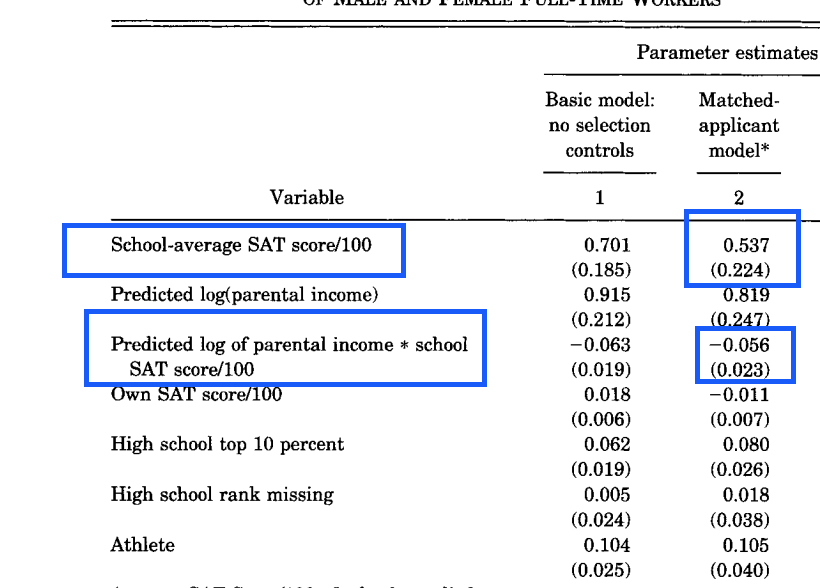
\includegraphics[width = 0.5\linewidth]{dk-interactions}	
\end{center}
\pause
\begin{wideitemize}
\item In DK, students at the 10th percentile of family earnings have log parental income of 8.86 ($\approx \$7,000 $)

\item What is the estimated effect of going to a school w/avg SAT 100 points higher for students at the 10th percentile? 
\pause
$$\hat\beta_D + \hat\beta_{DX} x  = \pause{} 0.537 - 0.056 \times 8.86 = 0.041$$


\end{wideitemize}
\end{frame}


\begin{frame}
	\begin{center}
		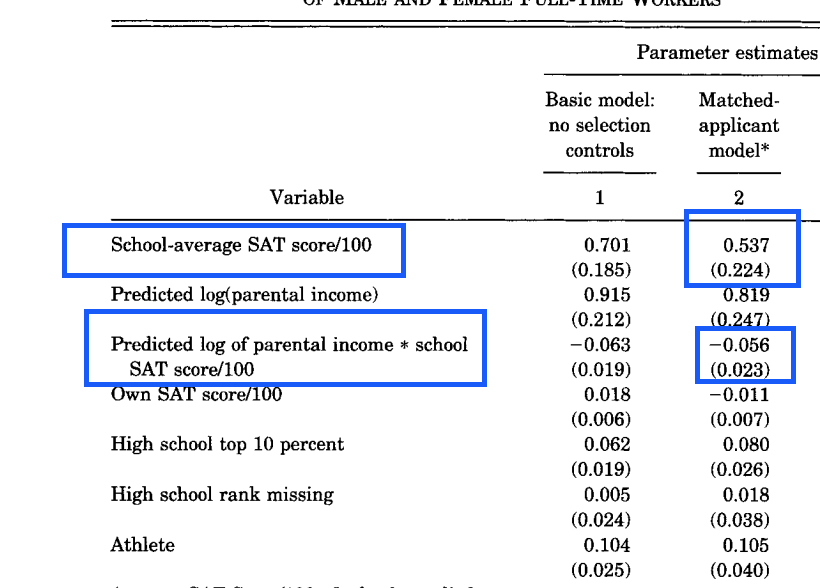
\includegraphics[width = 0.5\linewidth]{dk-interactions}	
	\end{center}
	\begin{wideitemize}
		
		\item  In DK, students at the 50th percentile of family earnings have log parental income of 10.39 ($\approx \$33,000 $)
		
		\item What is the estimated effect of going to a school w/avg SAT 100 points higher at the median? 
		$$\hat\beta_D + \hat\beta_{DX} x  = \pause{} 0.537 - 0.056 \times 10.39 = -0.045$$		
	\end{wideitemize}
\end{frame}


\begin{frame}{Explaining Heterogeneity}
	\begin{wideitemize}
		\item
		The results above showed that the returns to more selective college are positive for poorer students but negative for richer students
		
		\pause
		\item What might explain why elite college seems to matter more for students from poor backgrounds? \pause
		
		\item
		Not entirely clear... networking more important for students who don't have as many family connections?
	
		
	\end{wideitemize}
\end{frame}


\begin{frame}{Linear Combinations of Coefficients}
	\begin{wideitemize}
		\item
		In the DK example above, the estimated $CATE(x)$ for students with family income $x$ was $\hat\beta_D+ \hat\beta_{DX} x$.
		
		\pause
		\item
		Suppose we want to construct a CI or test hypothese about $CATE(x)$. How can we do that?
		
	\end{wideitemize}
\end{frame}


\begin{frame}{Linear Combinations of Coefficients}
	\begin{wideitemize}
		\item
		We showed several lectures ago that 
		
		$$\sqrt{N} (\bm{\hat\beta} - \bm\beta ) \rightarrow_d \mathrm{N}(\bm{0}, \bm{\Sigma}) $$
		
		\pause
		\item
		Say we're interested in $\beta_1 + \beta_2 x$. \pause{} Since $g(\bm{\beta}) = \beta_1 + \beta_2x$ is continuous, by the continuous mapping theorem we have \pause{}
		
		$$\sqrt{N}( \hat\beta_1 + \hat\beta_{2} x- ( \beta_1 + \beta_{2} x)) \rightarrow_d \mathrm{N}(0, \sigma_x^2) ,$$
		
		\noindent where $\sigma_x^2 = \Sigma_{11} + x^2 \Sigma_{22} + 2 x \Sigma_{12}$.
		
		
		\pause
		\item
		In previous classes we derived formulas for $\hat{\bm{\Sigma}}$, a consistent estimator of $\bm{\Sigma}$ (plugging in sample analogs) 
				
		\pause
		\item
		So we can form a CI for $\beta_1 + \beta_2 x$ using $\hat\beta_1 + \hat\beta_2 x \pm 1.96 \hat\sigma_x / \sqrt{N}$, where $\hat{\sigma}_x^2 = \hat\Sigma_{11} + x^2 \hat\Sigma_{22} + 2 x   \hat\Sigma_{12}$.
	\end{wideitemize}
\end{frame}


\begin{frame}{Example}
\begin{wideitemize}
\item
Recall that in DK we have $\hat\beta_D = 0.537$ and $\hat\beta_{DX} = -0.056$.

\item
Suppose that the part $\bm{\hat\Sigma}/N$ corresponding w/the coefficients of interest is

\begin{tabular}{l|rr}
& $\hat\beta_{D}$ & $\hat\beta_{DX}$ \\ \hline 
$\hat\beta_{D}$  & 0.0050  & -0.0025 \\
$\hat\beta_{DX}$ & -0.0025 & 0.0005
\end{tabular}
 
[Note: I had to make up the covariance term -- not in the paper] 
 
 \pause
 \item
 Then $\hat\Sigma_{11}/N = \pause{} 0.0050$, \pause $\hat\Sigma_{22}/N = \pause{} 0.0005$, \pause ,and $\hat\Sigma_{12}/N = \pause{} -0.0025$.
 
 \pause
 \item
 So a CI for $CATE(10.39)$ is \pause{}
\begin{align*}
&\beta_{D} + \beta_{DX} x \pm  1.96 \sqrt{ \hat\Sigma_{11}/N + x^2 \hat\Sigma_{22}/N +   2x \hat\Sigma_{12}/N } = \pause{} \\
&(0.537-0.056 \times 10.39) \pm \\ &1.96 \times \sqrt{  0.0050 + 10.39^2 \times 0.0005 + 2 \times 10.39 \times (-0.0025)  } = \pause \\
&[-0.21, 0.12]
\end{align*} 
 
\end{wideitemize}	
	
\end{frame}


\begin{frame}{lincom}
	\begin{wideitemize}
		\item
		The \texttt{lincom} command in Stata generalizes the argument above to test for any linear combination of coefficients, i.e. parameters of the form $a_1 \beta_1 + ...+ a_k \beta_k$
		

		\pause
		\item
		Similar (but slightly more complicated) asymptotic arguments can be used to test hypotheses on non-linear combinations of coefficients, e.g. $\beta_1 \beta_2 + \beta_3^2$. This can be done using the \texttt{nlcom} command in Stata.
	\end{wideitemize}
\end{frame}

	\begin{frame}{Outline}

	\textcolor{red!75!green!50!blue!25!gray}{1. Deriving Multivariate Regression and OLS}$\checkmark$
	\vspace{0.8cm}
	
	\textcolor{red!75!green!50!blue!25!gray}{2. Regression and Causality}$\checkmark$
	\vspace{0.8cm}
	
	3. Regression Odds and Ends
	
	\end{frame}

\begin{frame}{Odds and Ends 1: Multiple Hypothesis Testing}
	\begin{wideitemize}
		\item
		We've seen how to test for differences in causal effects across groups
		
		\pause
		\item
		We considered one dimension of heterogeneity: poor vs. rich students. But we might be interested in heterogeneity for other groups too\smallskip
			\begin{itemize}
				\item
				Are the effects bigger for men than for woman? \smallskip
				
				\pause
				\item
				Are the effects bigger for athletes than non-athletes? \smallskip
				
				\pause
				\item
				Are the effects bigger for male athletes from rich families than female non-athletes from poor families? 	
		   \end{itemize}
	   
	  \pause
	  \item
	  There are a large number of hypotheses that we may want to test! 	
	  
	  \pause
	  \item
	  This can lead to what's called a \textbf{multiple hypothesis testing} problem
	\end{wideitemize}	
\end{frame}


\begin{frame}{Multiple Hypothesis Testing (Cont.)}
	\begin{wideitemize}
		\item
		Remember: we constructed $p$-values so that (asymptotically), we have $p<0.05$ only 5\% of the time under the null hypothesis of no treatment effect
		
		\pause
		\item
		Thus, if we test for a significant effect among the entire population, if there is truly no effect we should reject the null only 5\% of the time. 
		
		\pause
		\item
		But suppose we first test for a significant effect among men. \\
		And we then also test for a significant effect among women. 
		
		\pause
		\item
		If there is no significant effect among either group, what is the probability that we find at least one significant effect? 

	\end{wideitemize}
\end{frame}


\begin{frame}
	\begin{wideitemize}
		\item 
		Suppose the samples for men and women are drawn independently. 
		
		\item
		Let $N_{sig}$ be the number of significant results.
		\begin{align*}
		&P( N_{sig} \geq 1  ) = \pause{} 1 - P(N_{sig} =0)  \pause{} \\
		&= 1 - P(\text{female insig and male insig}) \pause{} \\
		& = 1 -P(\text{female insig}) P(\text{male insig}) \pause{} \\ 
		& = 1-.95^2 \pause{} =  0.0975
		\end{align*}
	
	\item
	So we'll find at least one significant effect almost 10\% of the time if there is no effect for either group
	
	\pause
	\item
	By the same argument, if we test the null for $k$ independent groups, and there is no true effect, we will reject the null with probability \pause $1 - 0.95^k$
\end{wideitemize}
\end{frame}


\begin{frame}
Probability of finding at least one subgroup with a signficant effect with $k$ independent groups (and zero treatment effect):	\\
		\begin{tabular}{rr}
		$k$& $1-0.95^k$ \\ \hline 
		1 & 0.05 \\
		2 & 0.0975 \\ \pause{}
		3 & \pause{} 0.1426 \\
		5 &\pause{} 0.2262 \\
		10 & \pause{} 0.4013\\
		100 & \pause{} 0.9941
	\end{tabular}

\end{frame}


\begin{frame}{Simulating Multiple Hypothesis Testing}
\begin{wideitemize}
	\item
	Have survey data on average hourly wages from the Current Population Survey
	
	\item
	I generate a fake treatment $D_i$ which is 1 with probability 1/2
	
	\pause
	\item
	What's the true causal effect of this treatment? \pause 0, of course
	
	\pause
	\item
	I simulate this fake treament 100 times, and estimate 
	
	\begin{enumerate}
		\item 
		The treatment effect pooling all states
		
		\item
		The individual treatment effect for the first 10 states in the data
		
		\item
		The individual treatment effect for all 50 states in the data
		
	\end{enumerate}

	\pause
	\item
	I then calculate the fraction of simulations in which we get at least one significant estimate

\end{wideitemize}	
	
\end{frame}


\begin{frame}
	\only<1-2>{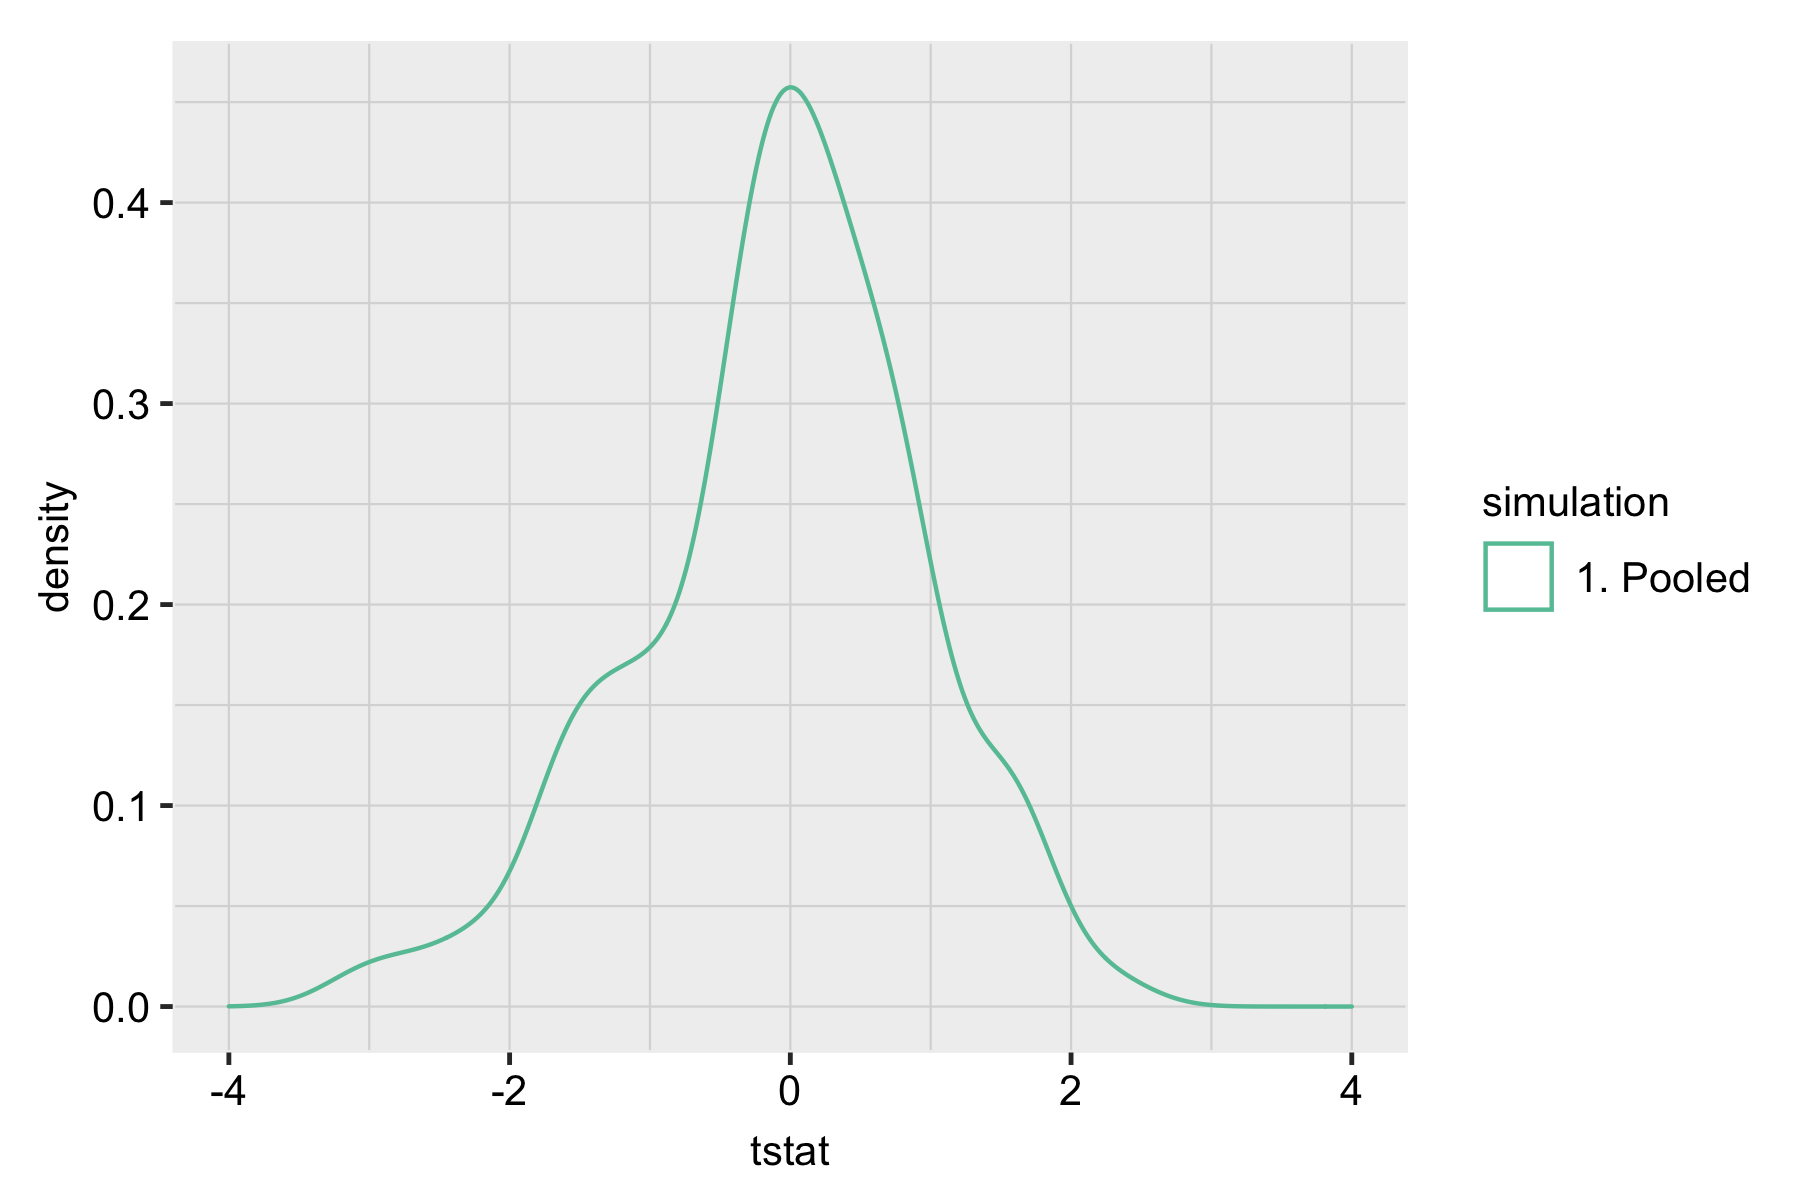
\includegraphics[width = 0.8\linewidth]{multiple-hypothesis-testing-pooled-only}}
	\only<3-4>{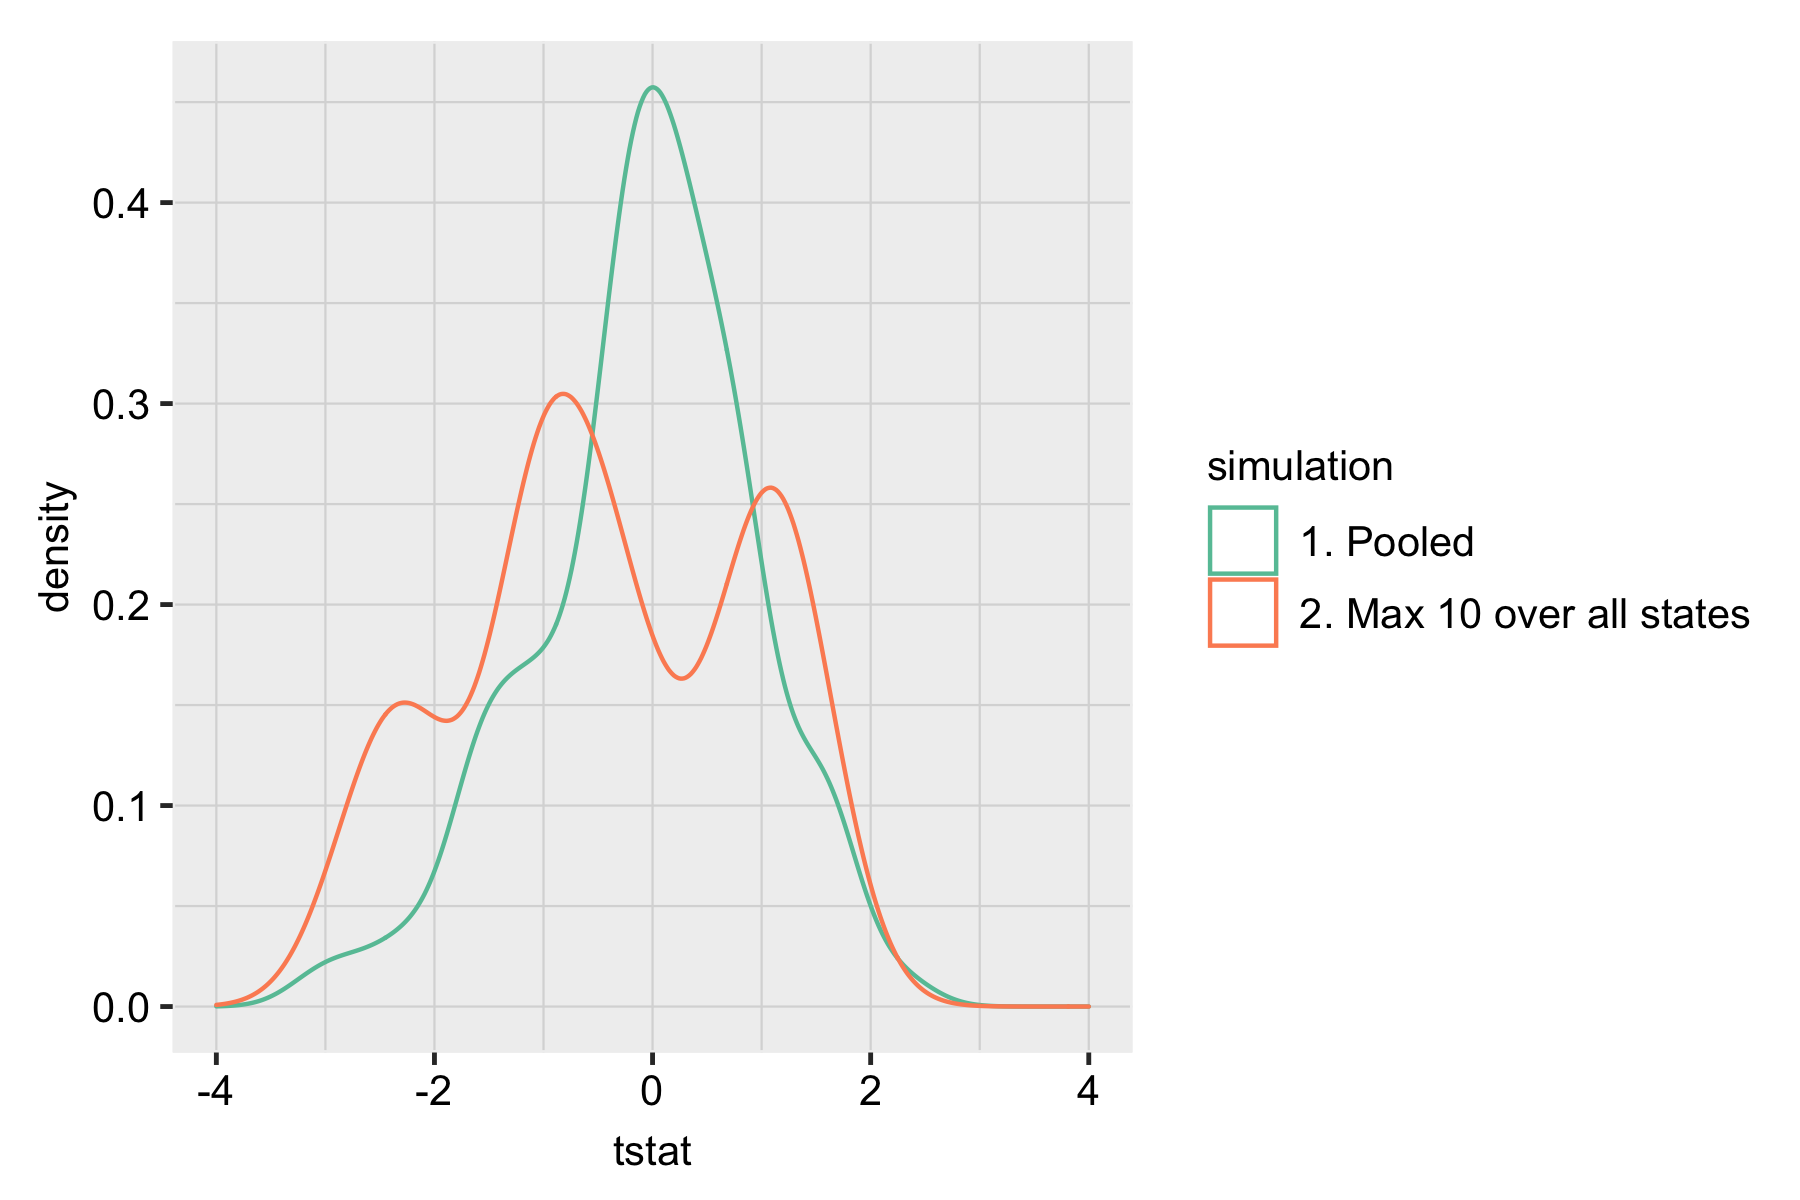
\includegraphics[width = 0.8\linewidth]{multiple-hypothesis-testing-pooled-plus-10}}
	\only<5-6>{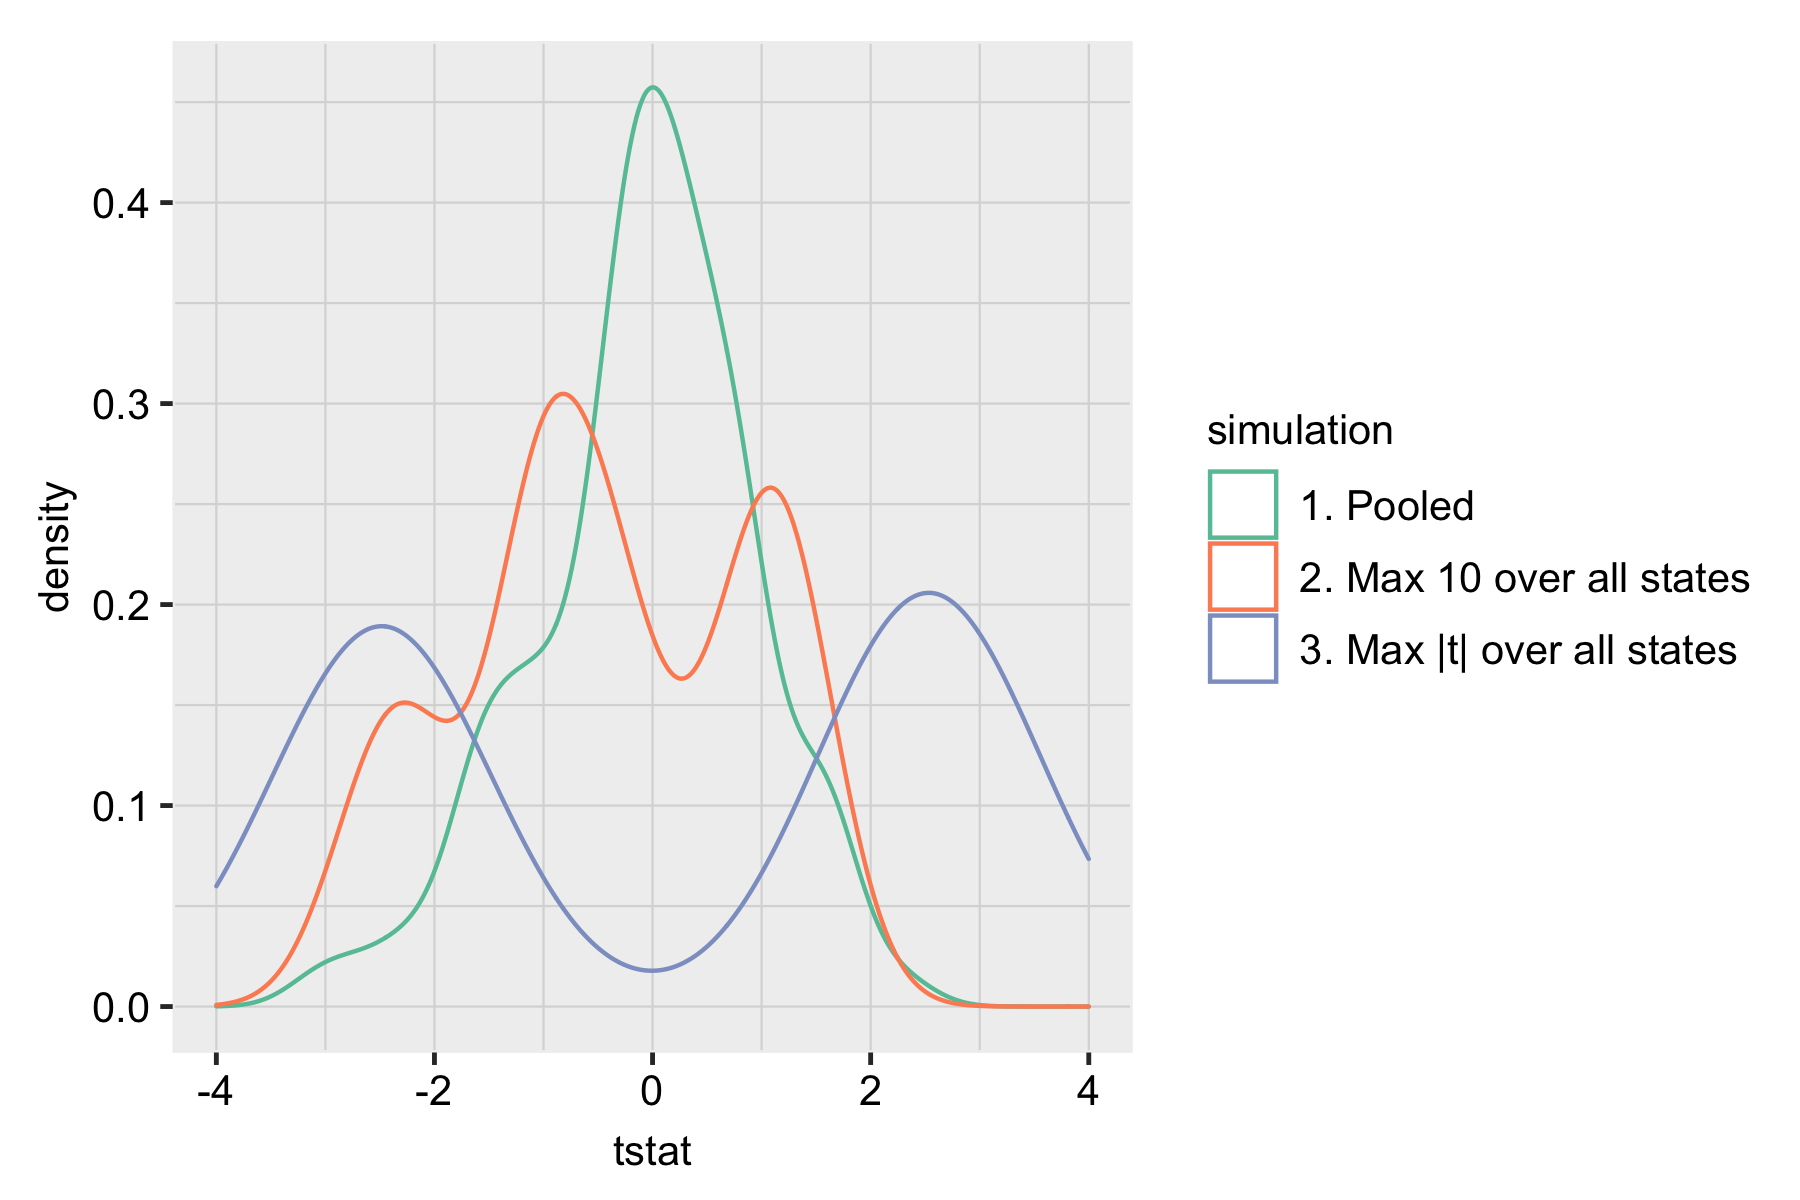
\includegraphics[width = 0.8\linewidth]{multiple-hypothesis-testing-all}}
	
	\only<2>{	
		\begin{wideitemizeshort}
			\item When testing the pooled effect across all states, we find a significant effect 5\% of the time
		\end{wideitemizeshort}
		}
	
		\only<4>{	
		\begin{wideitemizeshort}
			\item When testing the pooled effect across all states, we find a significant effect 19\% of the time
		\end{wideitemizeshort}
	}
	
	
	\only<6>{	
		\begin{wideitemizeshort}
			\item When testing the pooled effect across all states, we find a significant effect 90\% of the time
		\end{wideitemizeshort}
	}
	
\end{frame}

\begin{frame}{Correcting for Multiple Hypothesis Testing}
\begin{wideitemize}
	\item
	The simplest correction for multiple hypothesis testing is the \textbf{Bonferroni} correction
	
	\pause
	\item
	Instead of testing each of the $k$ individual hypotheses at the 5\% level, we test each one at the $5/k$\% level.
	
	\pause
	\item
	Then 
	$$P( N_{sig} > 0  ) \leq \sum_k P( \text{k is signficant}  ) = k (0.05/k) = 0.05 $$
	
	\pause
	\item
	This works even if the hypotheses are not independent, e.g. when you have overlapping groups (e.g., one group is all states, the second group is Rhode Island)
	
	\pause
	\item
	Downside: if you have lots of hypotheses, power against any one hypothesis can be low (e.g., 99.9\% confidence intervals are very wide).\\ \pause{}
	And the test is generally conservative in the sense that we find any significant effect $<5$\% of the time
		
\end{wideitemize}	
\end{frame}


\begin{frame}
	Probability of rejecting at least one hypothesis without and with Bonferroni correction \\
	\begin{tabular}{lrr}
		Simulation & Uncorrected & Corrected \\ \hline
		Pooled & 0.05 & 0.05 \\
		10 States & 0.19 &  0.00 \\
		50 States & 0.90 & 0.04
	\end{tabular}
\end{frame}


\begin{frame}{Odds and Ends 2: Joint Hypotheses}
	\begin{wideitemize}
		\item
		Sometimes we're happy to know whether there is an effect for \textit{any} subgroup (e.g. any state)
		
		\pause
		\item
		Can test the \textbf{joint null} that there is no treatment effect for every subgroup
		
		\pause
		\item
		If we reject, we conclude that there is strong evidence that the treatment effect is non-zero for at least one subgroup
		
		\pause
		\item
		How do we do this? 
		
	\end{wideitemize}	
\end{frame}

\begin{frame}
	\begin{wideitemize}
	\item
	We showed that $\sqrt{N} (\bm{\hat\beta} - \bm{\beta}) \rightarrow_d \mathrm{N}(\bm{0}, \bm{\Sigma})$
	
	\item
	From the continuous mapping theorem, we get that $X = \sqrt{N} \bm{\hat\Sigma}^{-\frac{1}{2}} (\bm{\hat\beta} - \bm{\beta}) \rightarrow_d \pause{} \mathrm{N}(\bm{0}, \bm{I})$.
	
	
	\item
	Applying the continuous mapping theorem again, we get that 
	$$F = \sum_k X_k^2 \rightarrow \sum_k Z_k^2, \text{ where } Z \sim \mathrm{N}(\bm{0}, \bm{I})$$
	
	\pause
	\item
	The sum of $k$ independent normals squared is called a \textit{chi-squared} distribution with $k$ degrees of freedom, denoted $\chi^2(k)$.
	
	\pause
	\item
	We can compare $F$ to the 95th percentile of the $\chi^2(k)$ distribution, and reject if it is larger. 
	
	\pause
	\item
	This is often called an \textit{F-test}.
	\begin{itemize}
		\item
		Sometimes the critical values use what's called an $F$-distribution, which is a slight modification to the $\chi^2(k)$ that corrects for small sample sizes
	\end{itemize}	
	\end{wideitemize}	
\end{frame}

\begin{frame}
	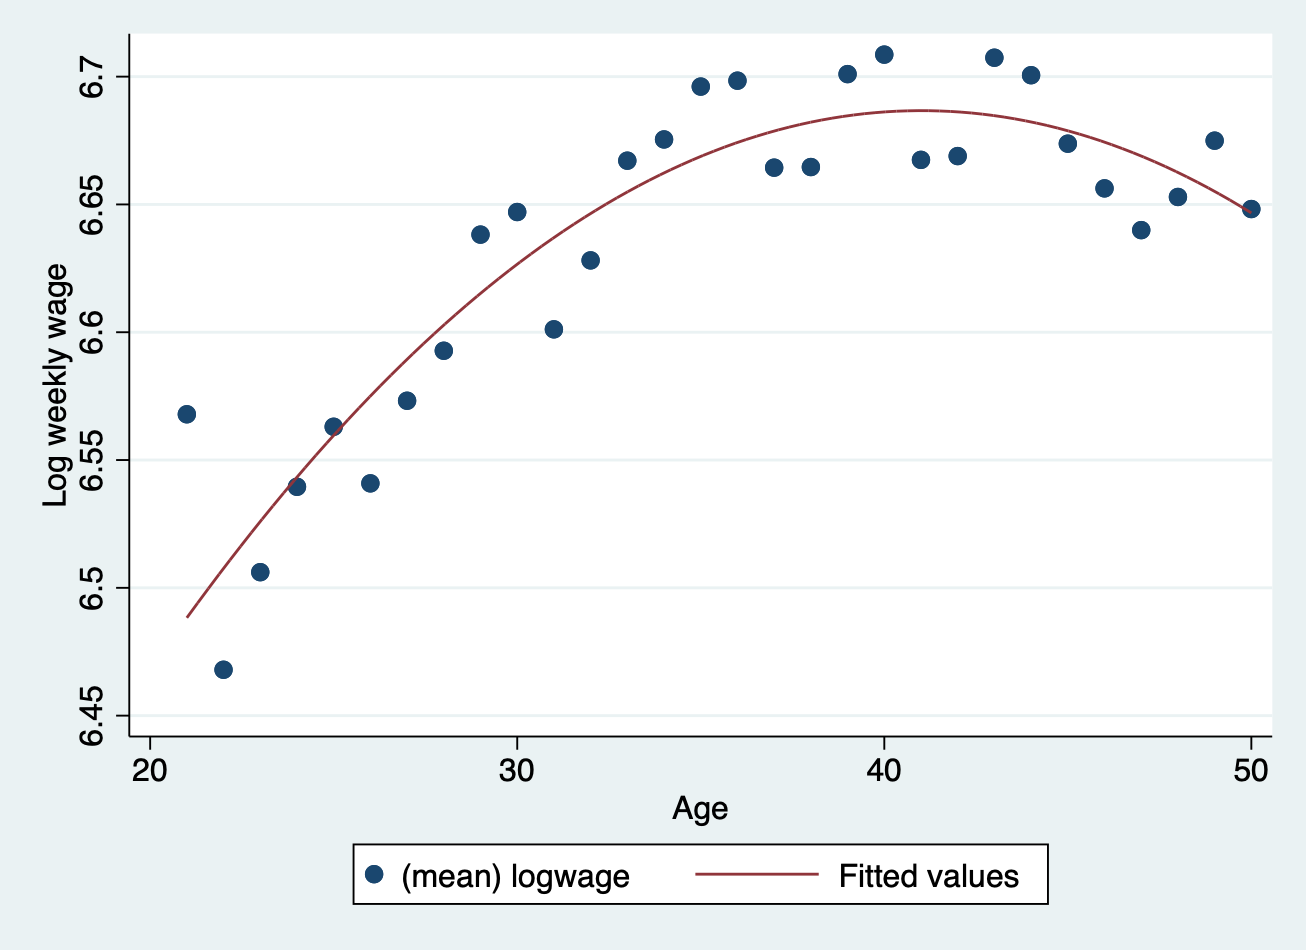
\includegraphics[width = 0.7\linewidth]{logwages-quadratic}
\end{frame}

\begin{frame}
	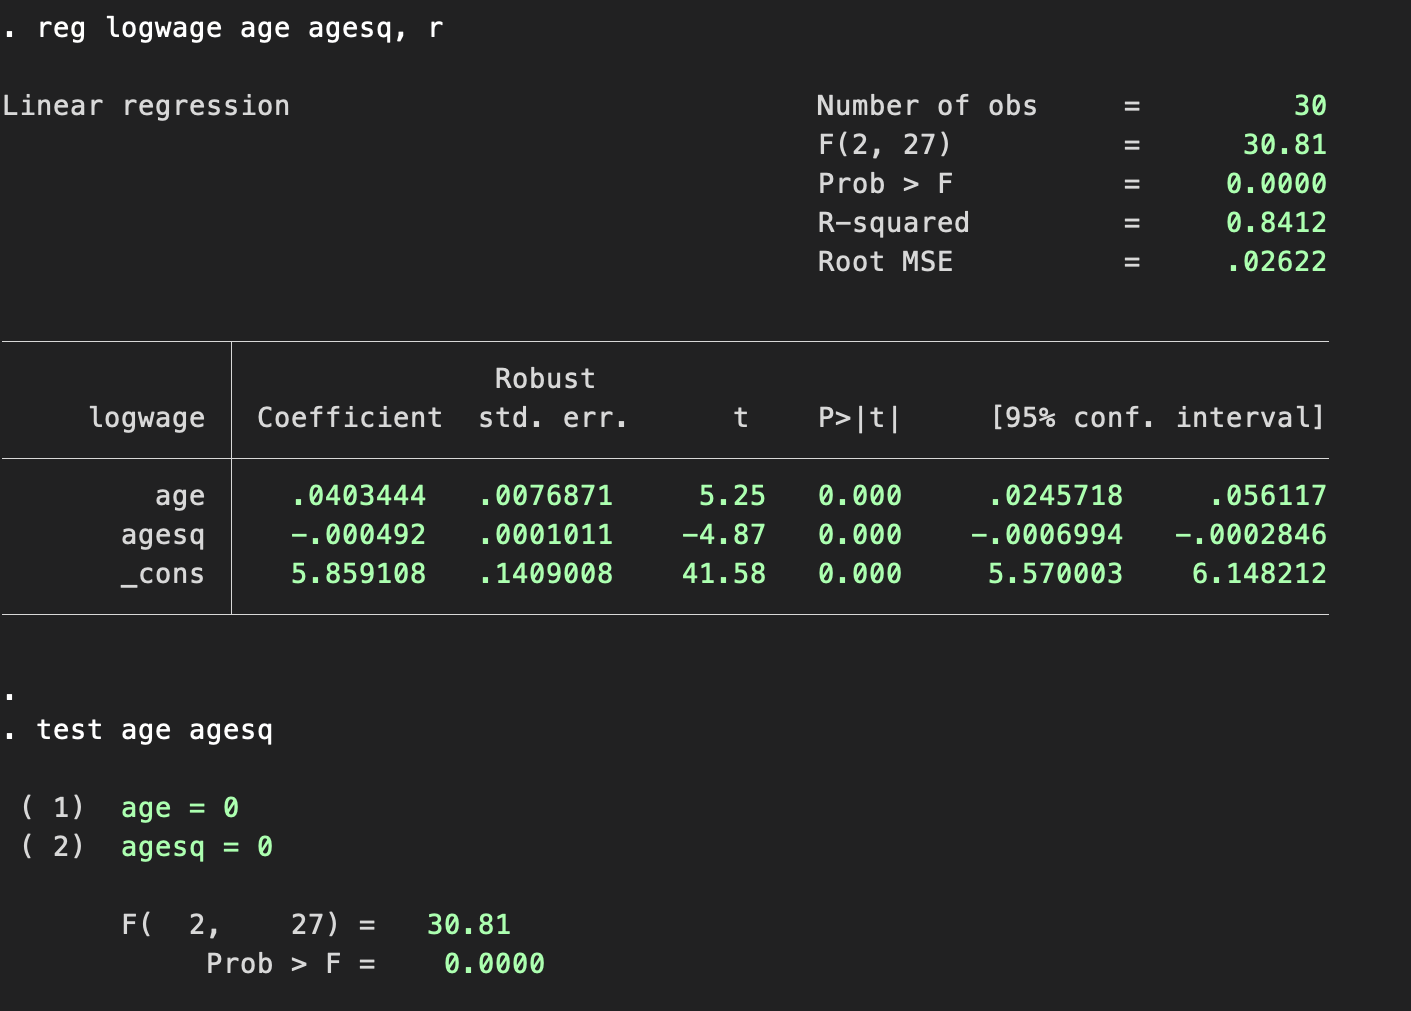
\includegraphics[width = 0.7\linewidth]{f-test}
\end{frame}


	
\end{document}


